%\documentclass[12pt]{article}
%\usepackage{amsmath}
%\usepackage{graphicx, color}
%\usepackage{amssymb}
%\usepackage{listings} %source code listing
%\usepackage{multirow}
%%\usepackage[version=2]{mhchem}
%\usepackage{subfig}
%\usepackage{hyperref}
%\usepackage{units}
%\usepackage{gensymb}
%\usepackage{adjustbox}
%\usepackage{listings}
%\usepackage{color}
%\usepackage{tcolorbox}
% 
%\definecolor{codegreen}{rgb}{0,0.6,0}
%\definecolor{codegray}{rgb}{0.5,0.5,0.5}
%\definecolor{codepurple}{rgb}{0.58,0,0.82}
%\definecolor{backcolour}{rgb}{0.95,0.95,0.92}
%
%\newcommand{\specialcell}[2][c]{%
%  \begin{tabular}[#1]{@{}c@{}}#2\end{tabular}}
% 
%
%
%\title{Reactor physics with Python \\ Lecture Notes}
%
%
%\author{Zs.~Elter. E. Branger, M. Preston \\ Uppsala University \\
%        Division of Applied Nuclear Physics}%\corref{cja}}
%%
%\date{2021.}
%\begin{document}

\section{Fission chain reaction and the energy distribution of neutrons}

The requirement to design a self-sustaining nuclear reactor is to achieve a balance in the production and loss of neutrons. This is often referred to as \textit{neutron economy}. As we will see later, the adequate way to study the neutron economy is by developing and solving the neutron transport equation. However, first in this chapter we will define the basic quantities of interest describing fission chain reactions, such as the multiplication factor. Then we will investigate the energy distribution of neutrons in traditional light water reactors and give a rather phenomenological description of the neutron transport process by studying the elements of the \textit{neutron cycle} from the birth of a neutron to its eventual death.


\subsection{Fission chain reaction}

As we discussed earlier the main principle of nuclear reactors that neutrons emerging from fission events are utilized to trigger further fission events, thus giving rise to a chain reaction. If one wants to have a steady chain reaction it needs to be sure that from each fission event on average only 1 neutron is going to cause a following fission event, and the rest of the neutrons are either captured in the reactor materials, or they leak out of the reactor. One common way to describe the fission chain reaction is by defining the \textit{multiplication factor k}:

\begin{equation}\label{eq:kdefault}
k=\frac{\text{Number of neutrons in \textit{i+1}th generation}}{\text{Number of neutrons in \textit{i}th generation}}
\end{equation}

where we define neutron generations: once a neutron triggers fission the new neutrons are considered to be in the next generation. If we follow several neutrons and the same time, and count the number of neutrons they give rise to, we can calculate $k$. Similarly we could have talked about the number of fission events instead. 

The multiplication factor $k$ can be

\begin{itemize}
\item $k<1$: the system is \textit{subcritical} (the number of neutrons decreases from generation to generation, the chain dies out)
\item $k=1$: the system is \textit{critical} (the number of neutrons is the same in each generation and stays always the same)
\item $k>1$: the system is \textit{supercritical} (the number of neutrons increases from generation to generation)
\end{itemize}

When operating the reactor, we usually wish to operate in critical conditions, when the number of neutrons, thus the fission rate, thus the power of the reactor is constant. Nevertheless, the reactor must be able to be supercritical (to increase the power to the required level) and subcritical (to decrease the power or to completely shut down the reactor) as well. Thus one needs to be able to control the reactor.

Nevertheless this often quoted life-cycle point of view definition of the multiplication factor Eq. \ref{eq:kdefault} can be misleading, and is also impractical. The fact is, that it is difficult to follow "one given" generation of neutrons. In fact, in a reactor several "neutron trees" develop at the same time, therefore it is difficult to tag them to decide which generation do they belong too. Also, Fig. \ref{fig:randomtrees} illustrates a simple case: a neutron has probability $p$ to enter fission, and it is lost from the chain otherwise, and in a fission $nu$ neutrons can be generated. A tree with critical conditions might die out, or grow exponentially, and in fact it will be only for the average of several trees that we can obtain the same number of neutrons in the succeeding generations. Of course, in a real nuclear reactor the number of neutrons are very high ($10^9$ neutron/cm$^3$), so we will in fact only see the average behavior. Lastly, what might be misleading here is that the time between the birth and death of a neutron is random (since it depends on the random path distance between collision, and on the number of scattering a neutron enters etc), thus neutrons of the same generation are not aligned so well in time as shown in Fig. \ref{eq:kdefault}. To summarize, care should be taken when thinking of the neutron transport in generations. 

\begin{figure}[ht!]
\protect \centering{
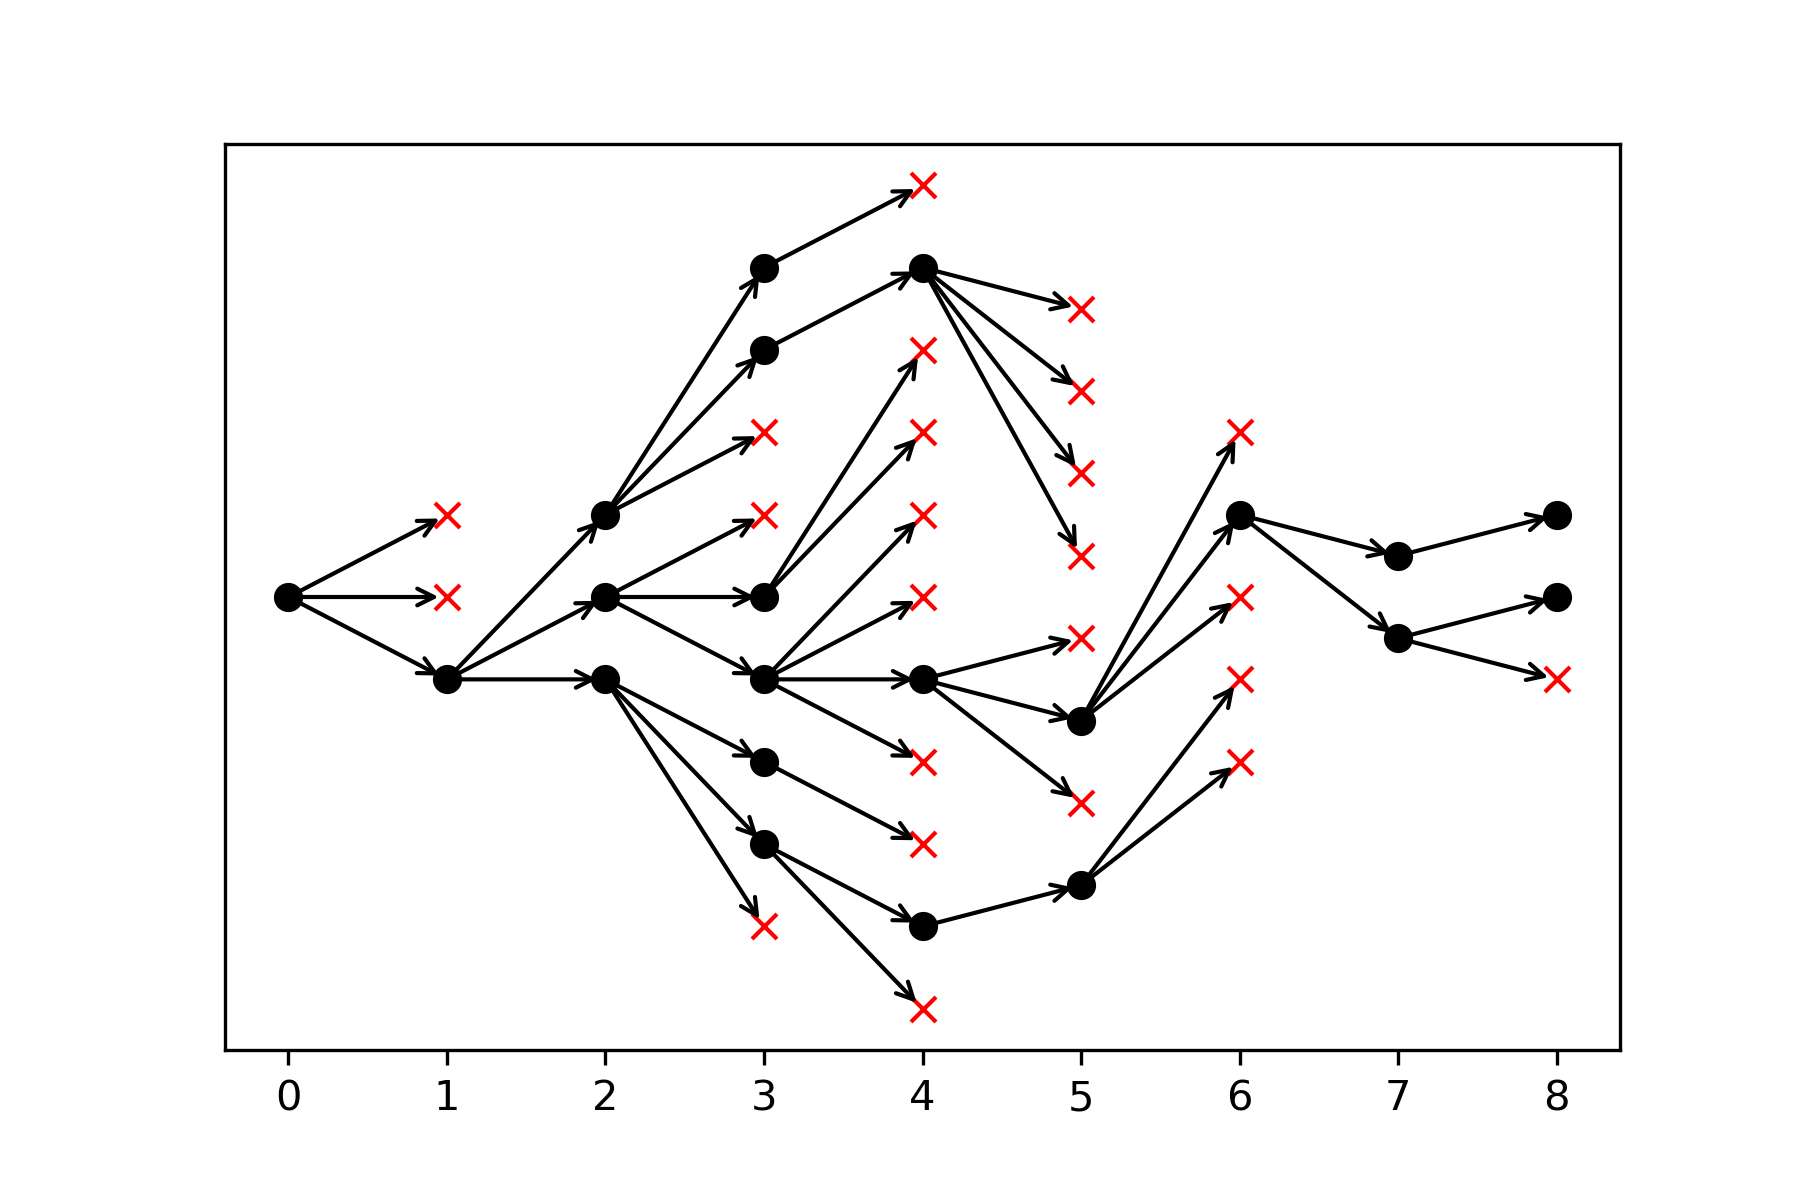
\includegraphics[scale=0.44] {figures/02-randomtreeC.png}
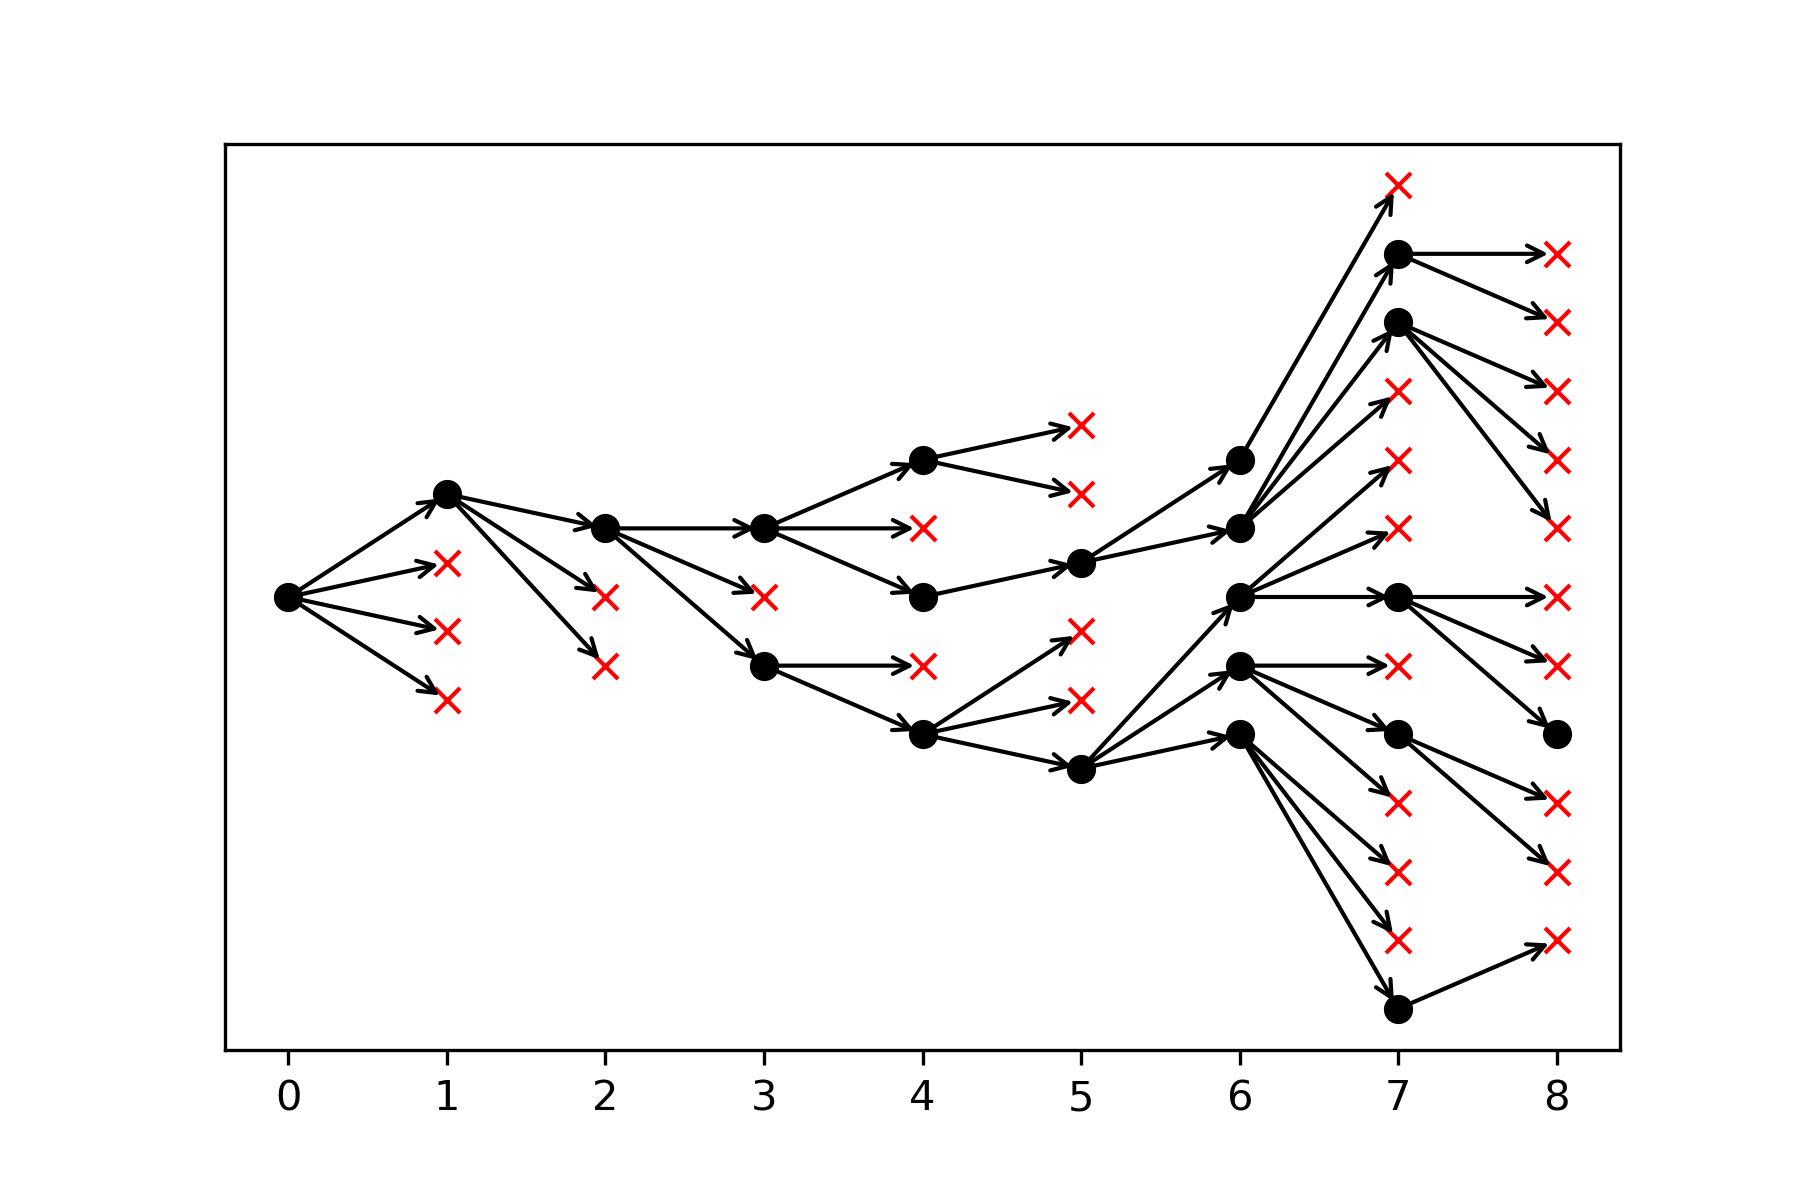
\includegraphics[scale=0.44] {figures/02-randomtreeD.png}
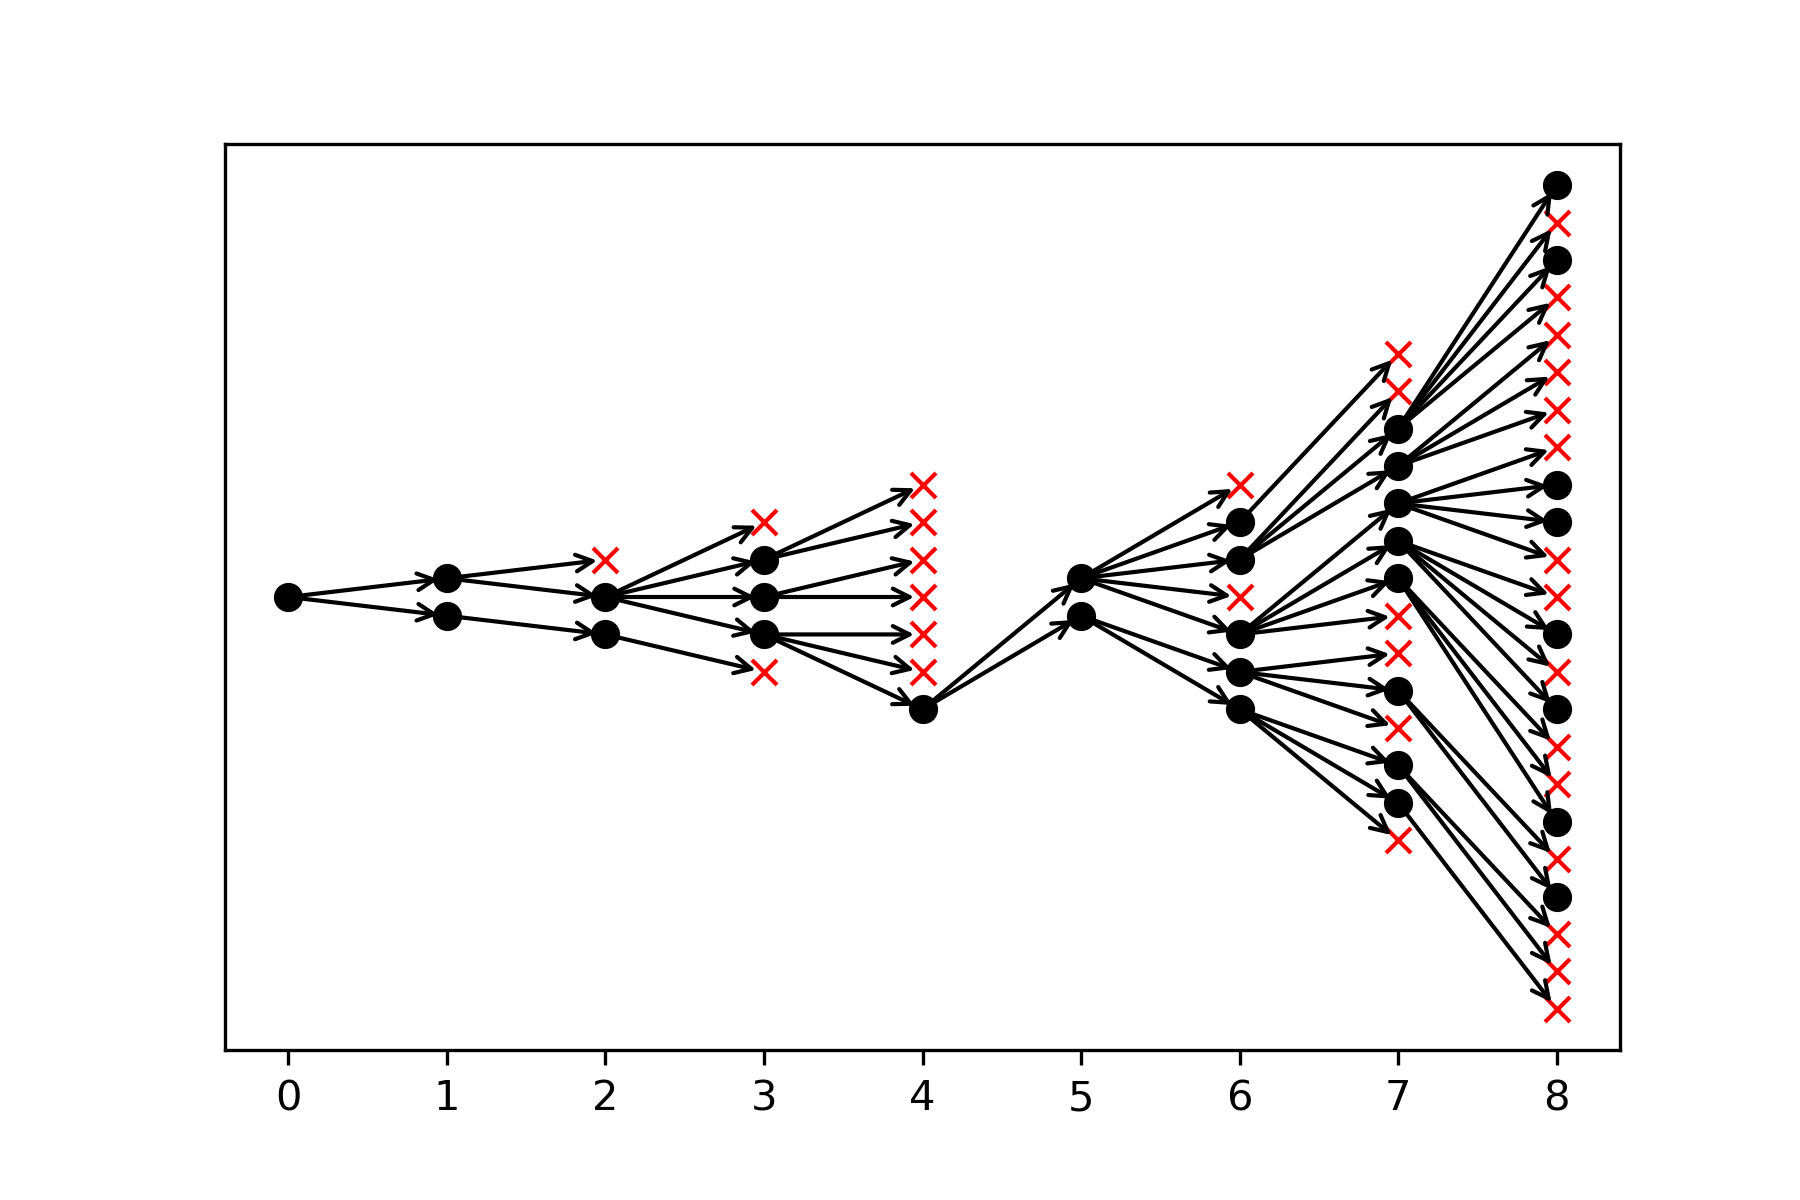
\includegraphics[scale=0.44] {figures/02-randomtreeE.png}
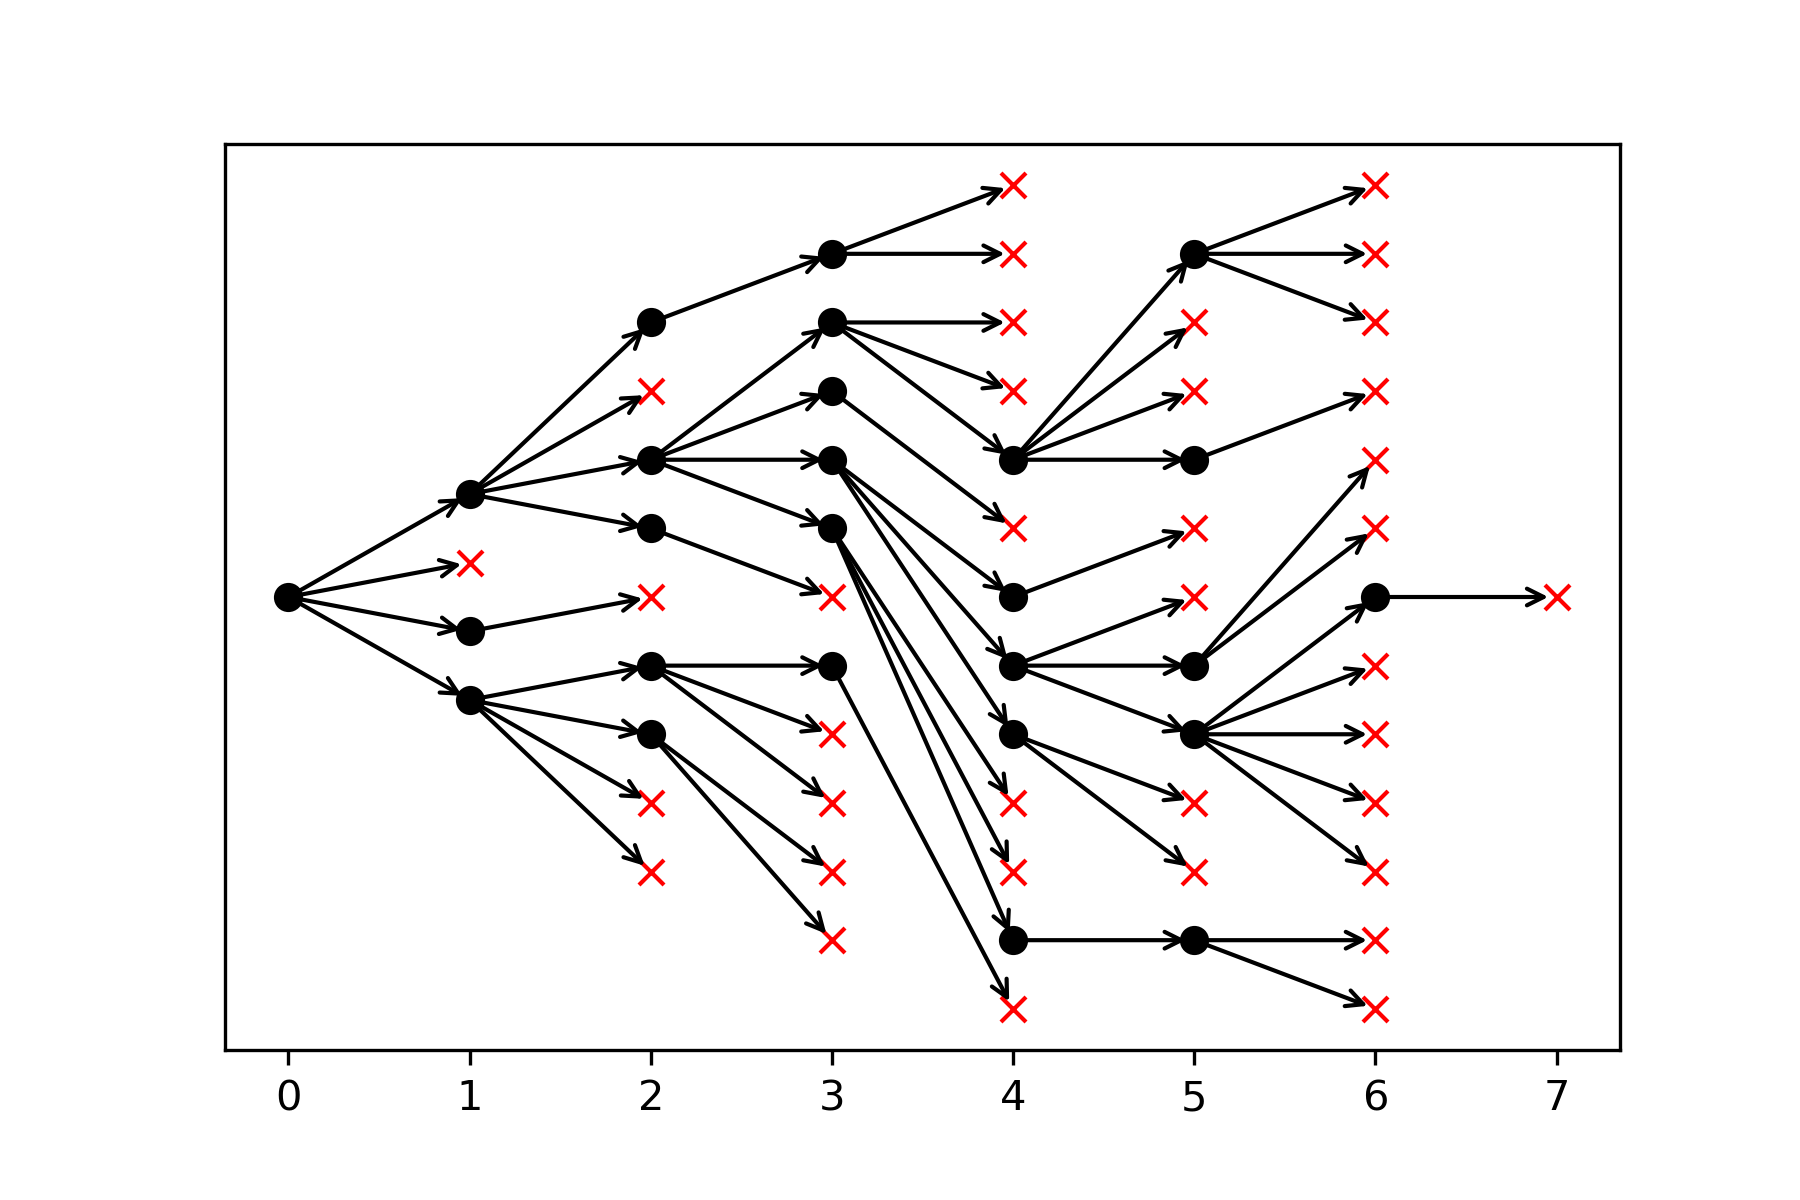
\includegraphics[scale=0.44] {figures/02-randomtreeF.png}}\protect
\caption{\label{fig:randomtrees} \footnotesize{Illustration of random critical trees.}}
\end{figure}

A slightly better and more practical way to define the multiplication factor is through production and loss rates, through the neutron balance (of course such rates also have some fluctuations, so here average rates are meant).

\begin{equation}\label{eq:krates}
k = \frac{\rm {Rate \: of \: neutron \: production}}{\rm Rate \: of \: neutron \: loss \: (absorption \: plus \: leakage) } = \frac{P(t)}{L(t)}
\end{equation}


\noindent where the time can be explicitly considered for the rates (eg. fuel evolution affects production rate, as we will see in later chapters). We will see later, that in fact we will to define the multiplication factor through reaction rates when developing equations to describe neutron transport. We can define the neutron lifetime as

\begin{equation}\label{eq:ell}
\ell=\frac{N(t)}{L(t)}
\end{equation}


\noindent where $N(t)$ is the total neutron population at time $t$. Note that $\ell L(t)$ is the number of lost neutrons during time $\ell$, thus in case $\ell$ is the mean lifetime of neutrons, all neutrons at time $t$ get lost over this time, while of course new neutrons are also generated.

\subsubsection*{Simple kinetics}

If we could somehow measure the exact number of neutrons at time $t$, then the change in $N(t)$ would be

$$\frac{dN}{dt}={\rm Production \: - Loss}=P(t)-L(t)$$

which can be rearranged with \eqref{eq:krates} and \eqref{eq:krates}

\begin{equation}
\frac{dN}{dt}=P(t)-L(t)=\Big(\frac{P(t)}{L(t)}-1 \Big)L(t)=\frac{k-1}{\ell} N(t)
\end{equation}

\noindent This equation we will see later can be derived more rigorously from the neutron diffusion equation. The solution of the equation is simply

\begin{equation}
N(t)=N(0)\exp\Bigg[\Bigg(\frac{k-1}{\ell}\Bigg)t\Bigg]
\end{equation}

\noindent where the value of $k$ will determine the number of neutrons overtime. In Fig. \ref{fig:basickinetics} one can see that for a supercritical system the average number of neutrons increases in time, for a critical system it stays constant and for subcritical system it decreases. This is in agreement with our previous definitions.

\begin{figure}[ht!]
\protect \centering{
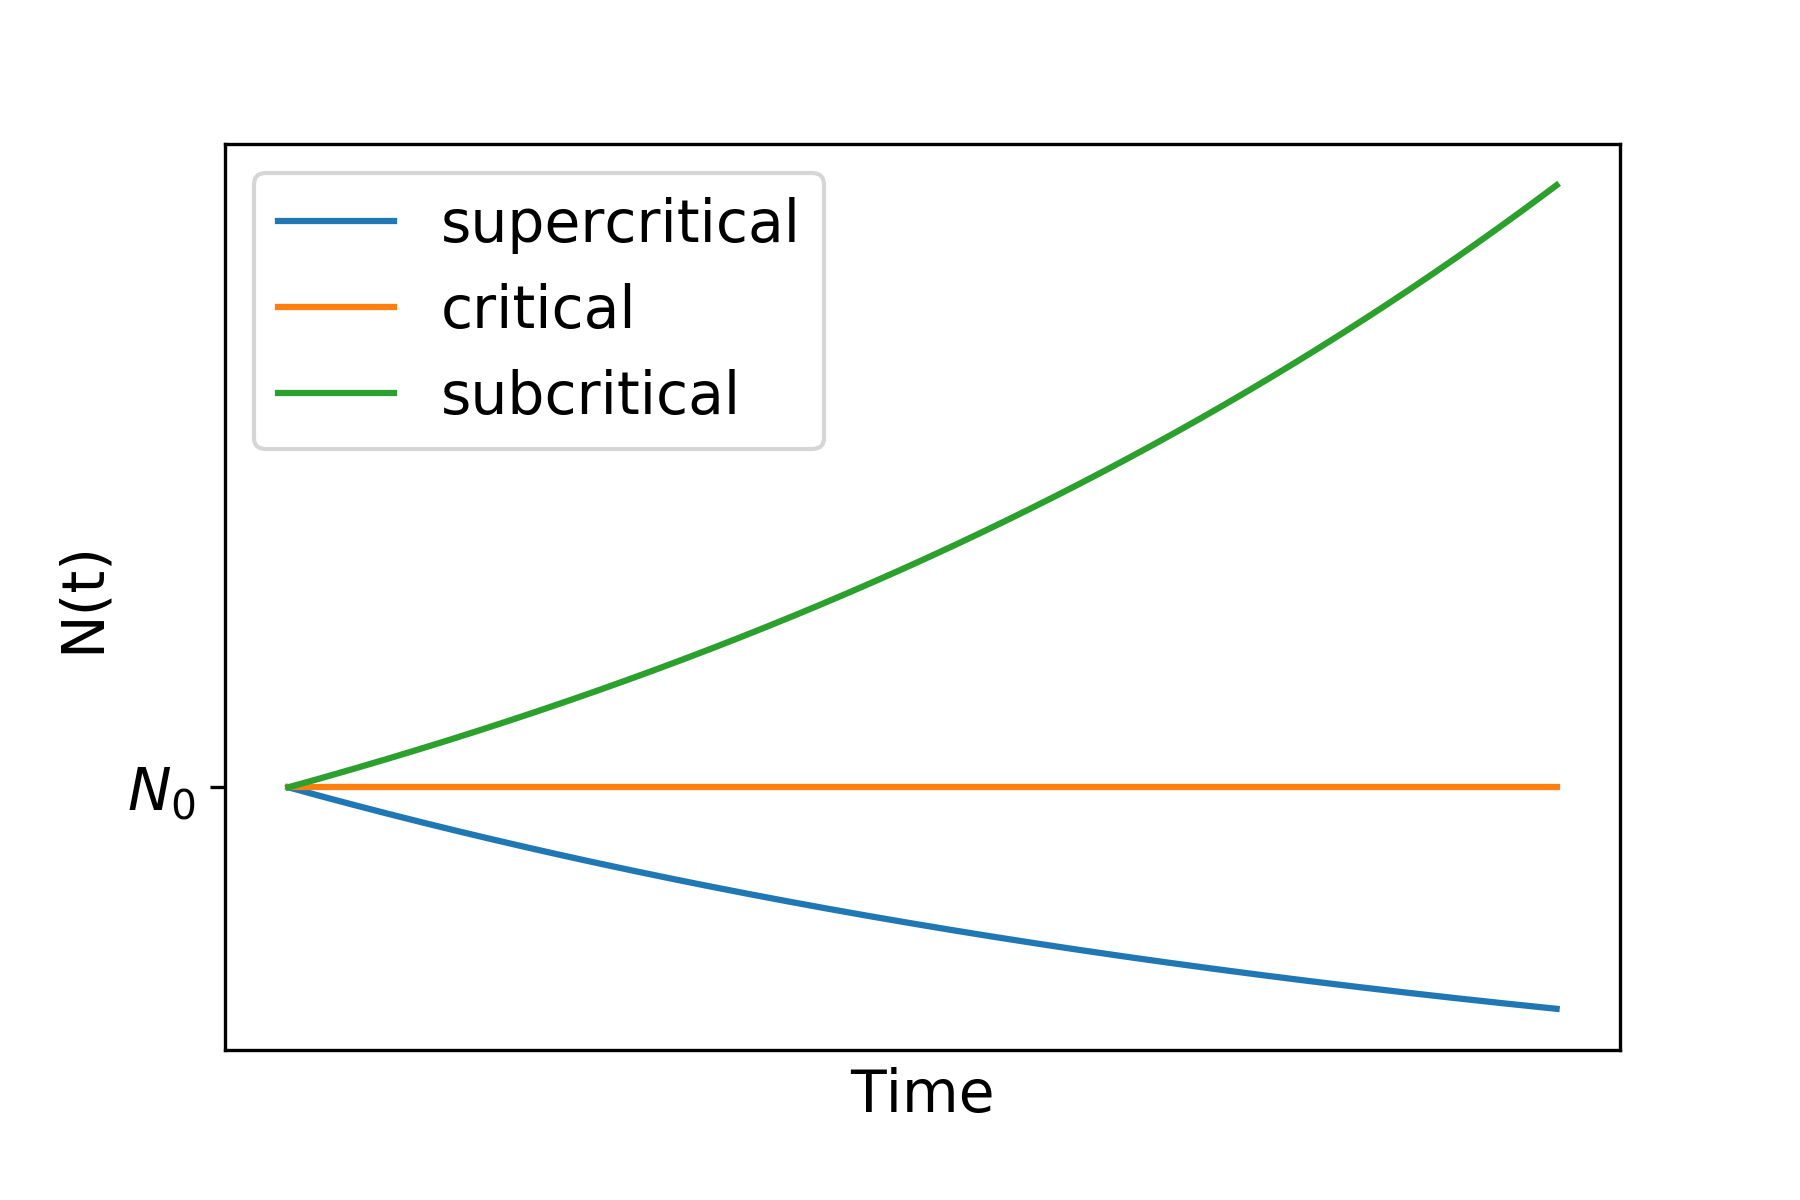
\includegraphics[scale=0.44] {figures/02-basickinetics.png}}\protect
\caption{\label{fig:basickinetics} \footnotesize{Number of neutrons over time.}}
\end{figure}

As a note we can mention here that the average neutron lifetime $\ell$ is around $10^{-4}s$, thus in a slightly supercritical system with $k=1.001$ the number of neutrons would increase by a factor of 22026 in a second. Such a small variation in the multiplication factor is very common in reactors, but such an increase would clearly not be controllable. But as we will see later, the presence of delayed neutrons does significantly increase the average lifetime of neutrons, and it makes the time behavior of reactors manageable.

\subsubsection*{2 factor formula}

Let us make a thought experiment in order to study the k-effective. Consider a homogeneous mixture of some nuclear fuel (uranium) and other cooling and structural materials. For our neutron trees in Figure \ref{fig:randomtrees} we considered that the neutron branch either dies out or initiates a fission event producing other neutrons. There are more way to die (or become irrelevant for the chain reaction) for a neutron. As illustrated in Figure \ref{fig:2factors}, there in fact, in a finite core the neutron either gets absorbed or leaves the system before interacting with it. Let's consider that the probability of non-leakage is $P_{NL}$. Then the neutron can be absorbed by a fuel nucleus or by some other nucleus (this is called \textit{parasitic capture}. Let's denote the conditional probability of the neutron being absorbed in fuel if it is absorbed with $P_{AF}$. Finally, the conditional probability if the neutron is absorbed in the fuel then it will initiate a fission event is $P_f$. After fission a number ($\nu$) of neutrons emerge.

\begin{figure}[ht!]
\protect \centering{
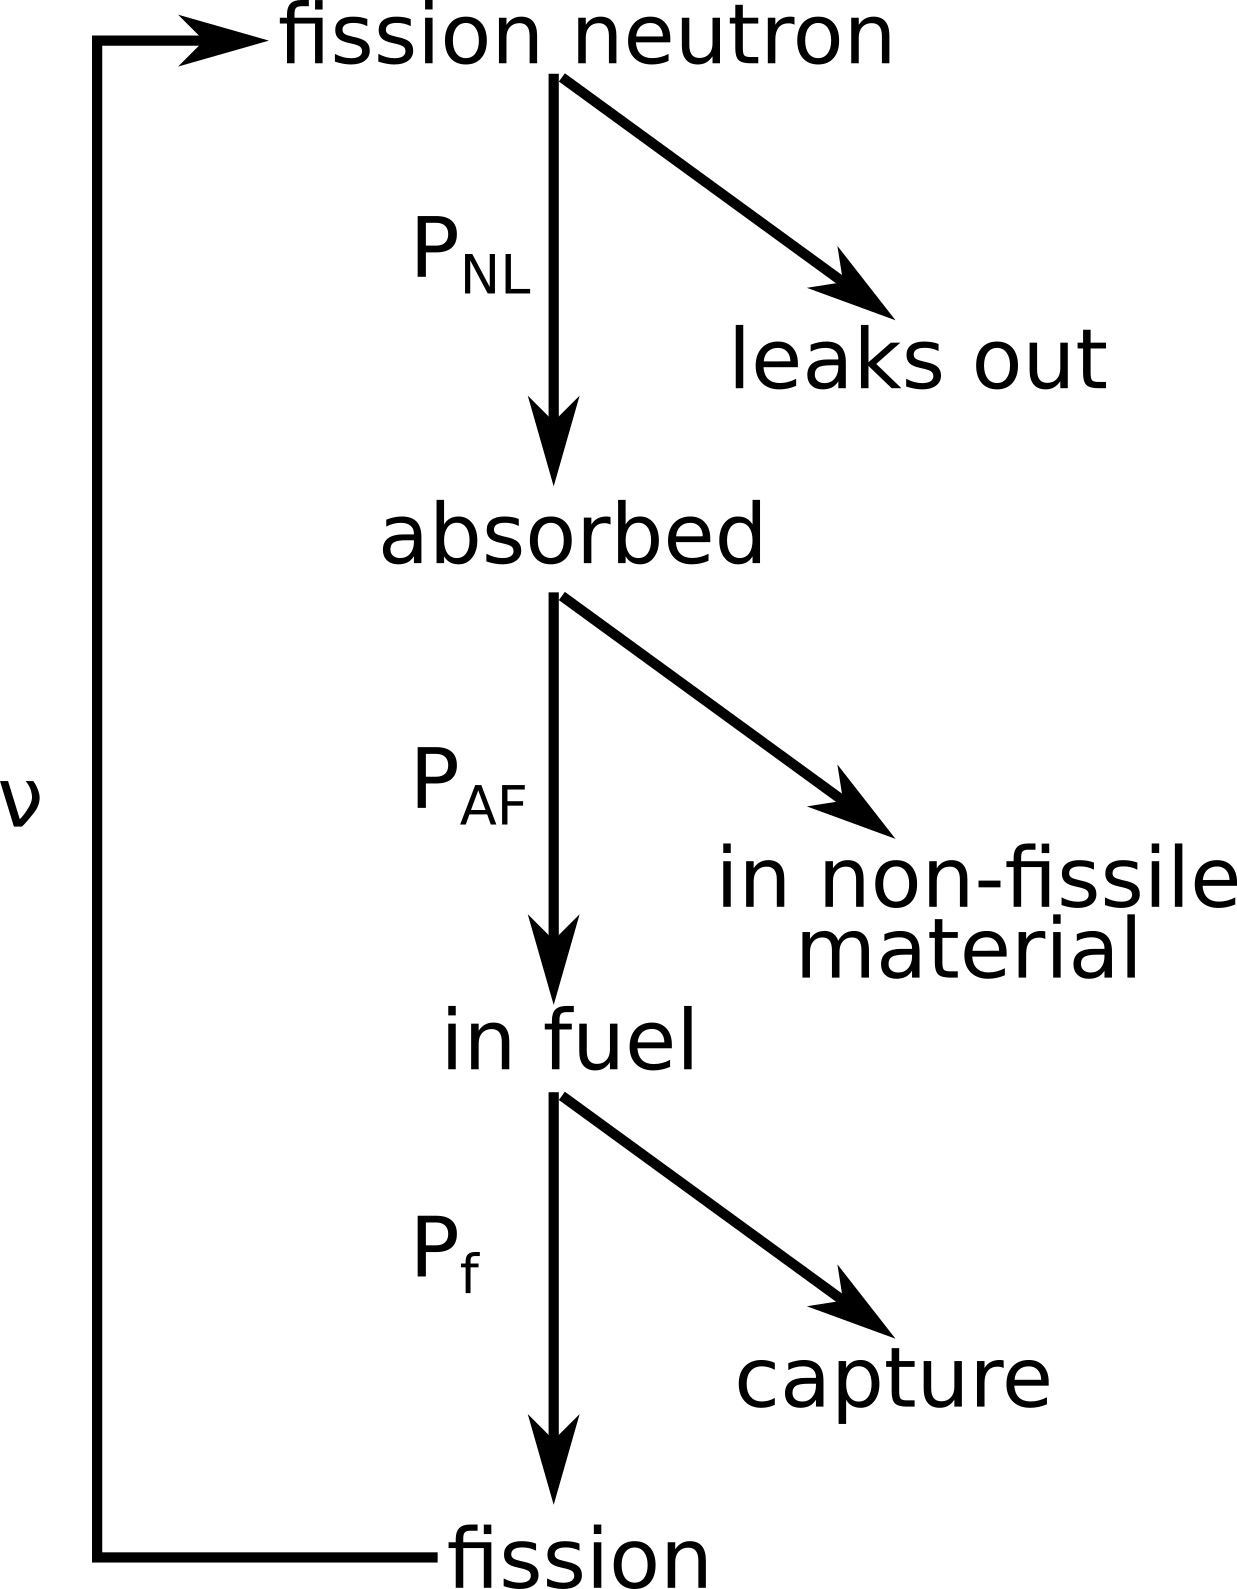
\includegraphics[scale=0.44] {figures/02-2factor.png}}\protect
\caption{\label{fig:2factors} \footnotesize{Probabilistic approach of understanding the multiplication factor.}}
\end{figure}

If $N_i$ neutrons started in a given generation, then it is easy to see that in the next generation the number of neutrons will be

$$N_{i+1}=\nu P_{NL}P_{AF}P_{f}N_i$$

therefore

$$k=\frac{N_{i+1}}{N_i}=\nu P_{NL}P_{AF}P_{f}$$

In order to assign actual physical quantities to these probabilities we have to remind ourselves that the cross sections of neutron-nucleus interactions characterized the probability of the event occurring. With little reasoning we can see that

$$f\equiv P_{AF} = \frac{\Sigma_a^F}{\Sigma_a}$$

\noindent where we introduced a new notation commonly used in the literature for the \textit{thermal utilization}. Similarly 

$$\eta \equiv \nu P_f= \nu\frac{\Sigma_f^F}{\Sigma_a^F}$$

\noindent where we found a quantity we have already looked upon, the \textit{thermal fission factor} or reproduction factor.

The non-leakage probability is more difficult to obtain, since it depends on the geometry of the core. Nevertheless, since $f$ and $\eta$ depend on the material properties only, often the infinite multiplication factor 

$$k_\infty=\eta f$$

is introduced to describe the multiplication of an infinite system (where neutrons cannot leak out). 

This simple model however does not account for the fact that in a thermal reactor the neutrons can have a wide range of energies, since they are born with energies in the order of MeV, however the fission reactions happen in the order of eV. Also, neutron cross sections have a strong dependence from the energy, as we saw earlier often with sudden jumps in the cross section. In order to refine our simple \textit{2 factor} model we will need to study the spectrum of neutrons.

\subsection{Neutron spectrum: Slowing down and thermalization}

With our previous studies we already have the intuition that neutrons can travel at very different speed in the reactor. They are born with relatively high (order of magnitude MeV) energies from fission, then they loose their energy in scattering reactions until they reach the thermal energies, when they can even gain energy from the nuclei of the medium. The energy distribution of the neutrons is called \textit{neutron spectrum}, and is defined as 

$$\Phi(E)=v(E)n(E) \: \Big[\frac{\text{n}}{\text{cm}^2\cdot\text{s}\cdot\text{eV}}\Big]$$

\noindent where $v(E)$ is the speed of neutrons and $n(E)dE$ is the number of neutrons in the energy interval $[E,E+dE]$. The main goal of this section is to determine $\Phi(E)$.

We can also recall that we have previously defined the reaction rate, and similarly we can define the spectral reaction rate quantities, eg. for some reaction$i$

$$R_i(E)=\Sigma_i(E)\Phi(E)$$

thus the total reaction rate is

$$R_i=\int_0^\infty\Sigma_i(E)\Phi(E)dE$$

In this section we will try to make a rough, quantitative analysis of the spectrum with the intention of introducing physical quantities relevant for the discussion of neutron slowing down and our goal will be to sketch the shape of the energy distribution. However we will neglect several aspects, for example space-dependent slowing down, and assume that the slowing down takes place in an infinite medium without spatial dependence.

Besides our curiosity, there is an other practical reason to calculate the neutron spectrum in a reactor: as we will see later, for the numerical treatment of neutron transport it is not possible to use the cross sections in their continuous form, instead we have to calculate weighted averages of the cross section, where the weighting function is going to be the spectrum. 

The difficulties to estimate the neutron spectrum arise from the fact that at various energies the phenomena at play to govern the transport of neutrons is different. Commonly, we separate three energy regions, which can be characterized with the following phenomena:

\begin{itemize}
\item Thermalization (0-1 eV): Upscattering due to thermal motion; Chemical binding and crystalline effects.
\item Slowing down or moderation (1-$10^5$eV): Elastic scattering from free nuclei at rest, isotropic in CM; Resolved resonances
\item Fast fission: Elastic scattering anisotropic in CM; inelastic scattering; Unresolved resonances
\end{itemize}

First we will introduce moderation (the slowing down of neutrons) in a rather heuristic way, and then we will study the spectrum at different energies.

\subsubsection{Moderation and moderators}

We can recall from the study of elastic scattering that the ratio of the neutron energy before ($E_i)$ and after scattering ($E_f$) is constant for a given CM scattering angle $\theta_C$:

\begin{equation}\label{eq:muErelation2}
\frac{E_f}{E_i}=\frac{(1+\alpha)+(1-\alpha)\cos\theta_C}{2}
\end{equation}

\noindent where $\alpha=(A-1)^2/(A+1)^2$, which means that the change of the logarithm of the energy is constant. We can define the average logarithmic decrement

\begin{equation}
\xi = \int\limits_0^{E_i}\ln\Big(\frac{E_i}{E_f}\Big)P(E_i\rightarrow E_f)dE_f=1+\frac{\alpha}{1-\alpha}\log\alpha \approx \frac{2}{A+2/3}
\end{equation}

\noindent where we introduced the scattering kernel from our previous studies, and the last approximation holds for not too small $A$.

In case of a homogeneous mixture of nuclides we can weight with the scattering cross section:

$$\bar\xi = \frac{\sum_i\xi_i\Sigma_{si}}{\sum_i\Sigma_{si}}$$

The value of $\xi$ characterizes how many scattering reactions are needed to slow down the neutrons. The larger the value of $\xi$ the less scattering is needed. Materials which is can efficiently slow down neutrons we call \textit{moderators}. The average number of collisions to slow a neutron from fast energies to thermal energies can be calculated with

$$\frac{1}{\xi}\ln(2 MeV/0.025 eV)=\frac{18.2}{\xi}$$

The ability of slowing down neutrons can be characterized with \textit{moderating power} $\xi\Sigma_s$: the logarithmic energy loss per distance traveled by the neutron. However, when assessing how good a moderator is, we have to consider also how much neutrons are absorbed by the moderator, therefore we can define the \textit{moderating ratio}

$$\xi\Sigma_s/\Sigma_a$$

\noindent As we see from Table \ref{tab:moderator}, the best moderators the ones containing low mass nuclei. However we can also notice, that even though hydrogen is the lightest, it is not the best moderator, when considering absorption as well. This is the reason that for a reactor moderated with light water one needs to enrich uranium in order to make it critical. However if a reactor is moderated with heavy water (such as the CANDU reactors) or graphite (such as the MAGNOX reactors), criticality can be achieved with natural uranium as well. There is obviously a compromise whether we spend our efforts on enriching the fuel, or producing heavy water. 


\begin{table}\caption{Moderating properties of various materials}\label{tab:moderator}
\begin{tabular}{c | c | c | c | c | c | c}
Moderator & $A$ & $\alpha$ & $\xi$ & $18.2/\xi$ & $\xi\Sigma_s (\text{cm}^{-1})$ & $\xi\Sigma_s/\Sigma_a$ \\
\hline
H & 1 & 0 & 1.0 & 18 & 1.3 & 61 \\
D & 2 & 0.111 & 0.725 & 25 & 0.08 & 2538 \\
Be-9 & 9 & 0.64 & 0.2 & 87 & 0.15 & 125 \\
C-12 & 12 & 0.716 & 0.158 & 115 & 0.061 & 190 \\
U-238 & 238 & 0.983 & 0.0084 & 2172 & 0.04 & 0.16
\end{tabular}
\end{table}

\subsubsection*{Lethargy}

When discussing slowing down it is often more natural to use an other variable than energy, the \textit{lethargy}, which often feels intimidating for novice reactor physicist. Although we promise we will not overuse it in this course, but since the reader will find this variable in other books, it is necessary to introduce it. The lethargy gives the logarithmic energy loss compared to some fix energy $E_0$:

$$u=\ln(E_0/E)$$

$$E=E_0\exp(-u)$$

\noindent where $E_0$ is typically the energy of the source or a sufficiently high energy (eg. 10 MeV) in case of fission sources). We can notice  that $\xi$ is the average increase of lethargy in a collision. The neutron flux therefore can be written as

$$\Phi (u)du=\Phi (u)dE/E=\Phi (E)dE$$

$$\Phi(u)=\Phi(E)E$$

Figure \ref{fig:lethargy} makes it even more apparent why working with the lethargy is more natural in slowing down. We can see that the collision density (as discussed soon) is constant. We can also notice that the lethargy is increasing during slowing down: as neutrons get slower they get more "lethargic".

\begin{figure}[ht!]
\protect \centering{
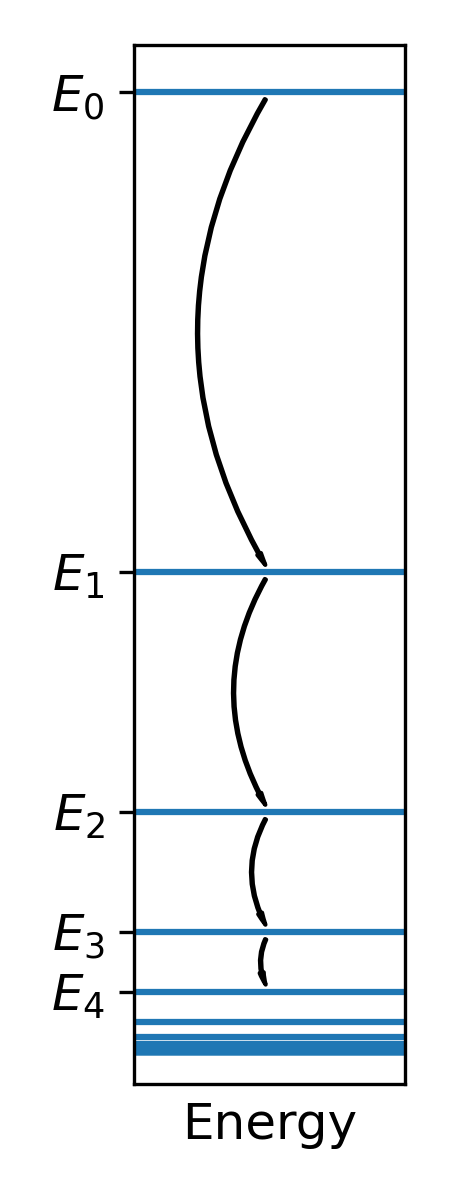
\includegraphics[scale=0.74] {figures/03-energychange.png}
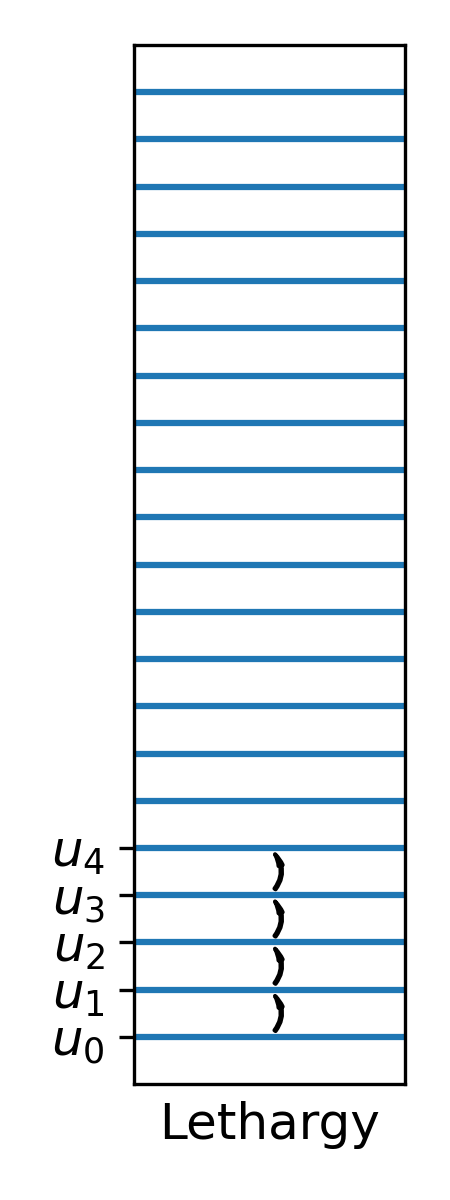
\includegraphics[scale=0.74] {figures/03-lethargychange.png}}\protect
\caption{\label{fig:lethargy} \footnotesize{Schematic illustration of energy and lethargy change during slowing down.}}
\end{figure}

\subsubsection{Neutron spectrum}

We will discuss the neutron spectrum in the three regions (thermal, moderate, fast) separately.

\subsubsection*{Fast and thermal region}

For the fast region we consider that the source of neutrons are the fission events, and little reactions happen to them, therefore the spectrum in this region can be well approximated with the Watt-spectrum. As we will see later in more realistic Monte Carlo calculation, although the shape indeed resembles the fission birth spectrum, but it is not entirely smooth.

For thermal energies, where neutrons can both loose or gain energy in scattering events, we can assume that the neutron spectrum follows the Maxwell-distribution

$$\phi(E)\propto E\exp\big(-\frac{E}{kT}\big)$$

\noindent although it has to be mentioned that in reality due to absorbing events taking place at these energies, the real neutron spectrum is slightly shifted to higher energies, this is called spectral hardening.

\subsubsection*{Slowing down region}

We will consider the slowing down in an infinite, homogeneous geometry and assume that the neutron source is spatially uniform. First, we will develop an equation describing the slowing down.

Let us notice that 

\begin{itemize}
\item $\Sigma_t(E)\Phi(E)dE$ is the number of collisions per unit time within $[E,E+dE]$ which removes neutrons from the energy interval.
\item $S(E)dE$ is the number of neutrons emitted per unit time within $[E,E+dE]$
\item $\int\limits_0^\infty \Phi(E')\Sigma(E'\rightarrow E)dE'dE$ is the number of neutrons per unit time reaching $[E,E+dE]$ through scattering
\end{itemize}

In case of steady state, we can assume that the source terms (the source and the in-scattering events) are in balance with the loss term (the total number of collisions removing neutrons from our energy interval):

\begin{equation}
\int\limits_0^\infty \Phi(E')\Sigma(E'\rightarrow E)dE'+S(E)=\Sigma_t(E)\Phi(E)
\end{equation}

\noindent is the \textit{slowing down equation} which as we will see in the next chapter could be derived directly from the general neutron transport equation.

Let us consider that inelastic scattering can be neglected for energies below 100 keV and elastic scattering can be considered isotropic in CM, and recall the scattering kernel for elastic scattering:\footnote{Note, that previously we used the $(E\rightarrow E')$ notation, since we were curious which energies are reached from our initial energy $E$, now we swapped the notation of initial and final energy, because we are more interested in which energies contribute to our final energy, and it is more convenient to develop the equation for variable $E$. Nevertheless the meaning is still the same: $E_{initial}\rightarrow E_{final}$}

\begin{equation}\label{eq:scatkernel}
    \Sigma_s(E'\rightarrow E) = 
    \begin{cases}
      \frac{\Sigma_s(E')}{(1-\alpha)E'} & \text{if} \: \alpha E' \leq E \leq E' \\
      0 & \text{otherwise}
    \end{cases}
\end{equation}

\noindent In case of a mixture of various nuclides the scattering kernel would be the sum of the scattering kernels of each nuclide. However, in practice usually there is one type of nuclide which has much better moderating properties than the others, thus we can neglect the contribution of the others. By substituting this kernel into the slowing down equation we arrive to

\begin{equation}\label{eq:slowingdown}
\int\limits_E^{E/\alpha} \Phi(E')\frac{\Sigma_s(E')}{(1-\alpha)E'}dE'+S(E)=\Sigma_t(E)\Phi(E)
\end{equation}

\noindent which looks fairly innocent, but in practice can be easily tackled only in a couple of situations:

\begin{enumerate}
\item Slowing down without absorption ($\Sigma_a=0 \rightarrow \Sigma_t=\Sigma_s$)
\item Slowing down on hydrogen nuclei with absorption
\item Slowing down on arbitrary nuclide but with energy independent cross sections
\end{enumerate}

Of course in practice the most important case would be to solve the equation for arbitrary nuclides and energy dependent cross sections, however for that case no analytic solution is available. In this lecture note we are going to discuss 1. and 2., since they will provide enough insight about the neutron spectrum in this region.

\vspace{0.5cm}

\textbf{Slowing down without absorber}

As we noticed earlier the energy lost during scattering is decreasing during slowing down, however the average increase of lethargy is independent of the lethargy. Thus the number of collisions per time and unit energy in the energy bin $[E,E+dE]$, the collision density $F(E)=\Sigma_t(E)\Phi(E)$ is increasing with decreasing $E$. However the number of collisions per unit time per unit lethargy is independent of $u$. Thus

$$F(u)=\Sigma_t(u)\Phi(u)=\Sigma_t(E)\Phi(E)E=c$$

\noindent if we substitute $\Sigma_t(E)\Phi(E)=c/E$ in Eq. \eqref{eq:slowingdown}, we will find that indeed it is a solution if $\Sigma_t=\Sigma_s$ and at energies below the energies of the source (ie. when S(E)=0).

We can obtain $c$ by noticing that the number of neutrons per unit time whose energy passes above a given lethargy is the same as the number of neutrons emitted per unit time since there is no absorption. The number of neutrons emitted per unit time is simply the integral of the source neutron spectrum.

$$S=\int\limits_{E_S}^\infty S(E)dE$$

\noindent where $E_S$ is the energy below which the source does not emit neutrons. 

And the number of neutrons passing lethargy $u$ per unit time is $c\xi$, since all the neutrons will pass lethargy $u$ which suffered a collision between $u$ and $u-\xi$, therefore we can conclude that\footnote{Notice that $c=F(u)$, the collision density. The collision density is defined so that $F(u)du$ gives the number of collisions within [u,u+du] therefore $\int\limits_{u-\xi}^u F(u)du$ is the number of neutrons passing lethargy $u$. Therefore $S=F(u)\xi=c\xi$ }

$$c\xi=S$$

$$\Phi(E)=\frac{S}{\xi E\Sigma_s(E)}=\frac{S}{\xi E\Sigma_t(E)}$$

\noindent therefore if we combine our comments on the thermal and fast regions with our recent findings, we can illustrated our idealized neutron spectrum in Figure \ref{fig:idealneutronspectrum}. Notice that we have plotted both $\Phi(E)$ and the lethargic spectrum $E\Phi(E)$. As we will see later, indeed this rough sketch explains the main features of our actual neutron spectra in thermal systems rather well.

It also needs to be highlighted again, that these results are valid only at energy regions below the source energy. This is often called \textit{asymptotic region}. It is also important to point out that the scattering cross section can be considered independent of energy in the slowing down region, therefore $\Phi(E)\propto 1/E$.

\begin{figure}[ht!]
\protect \centering{
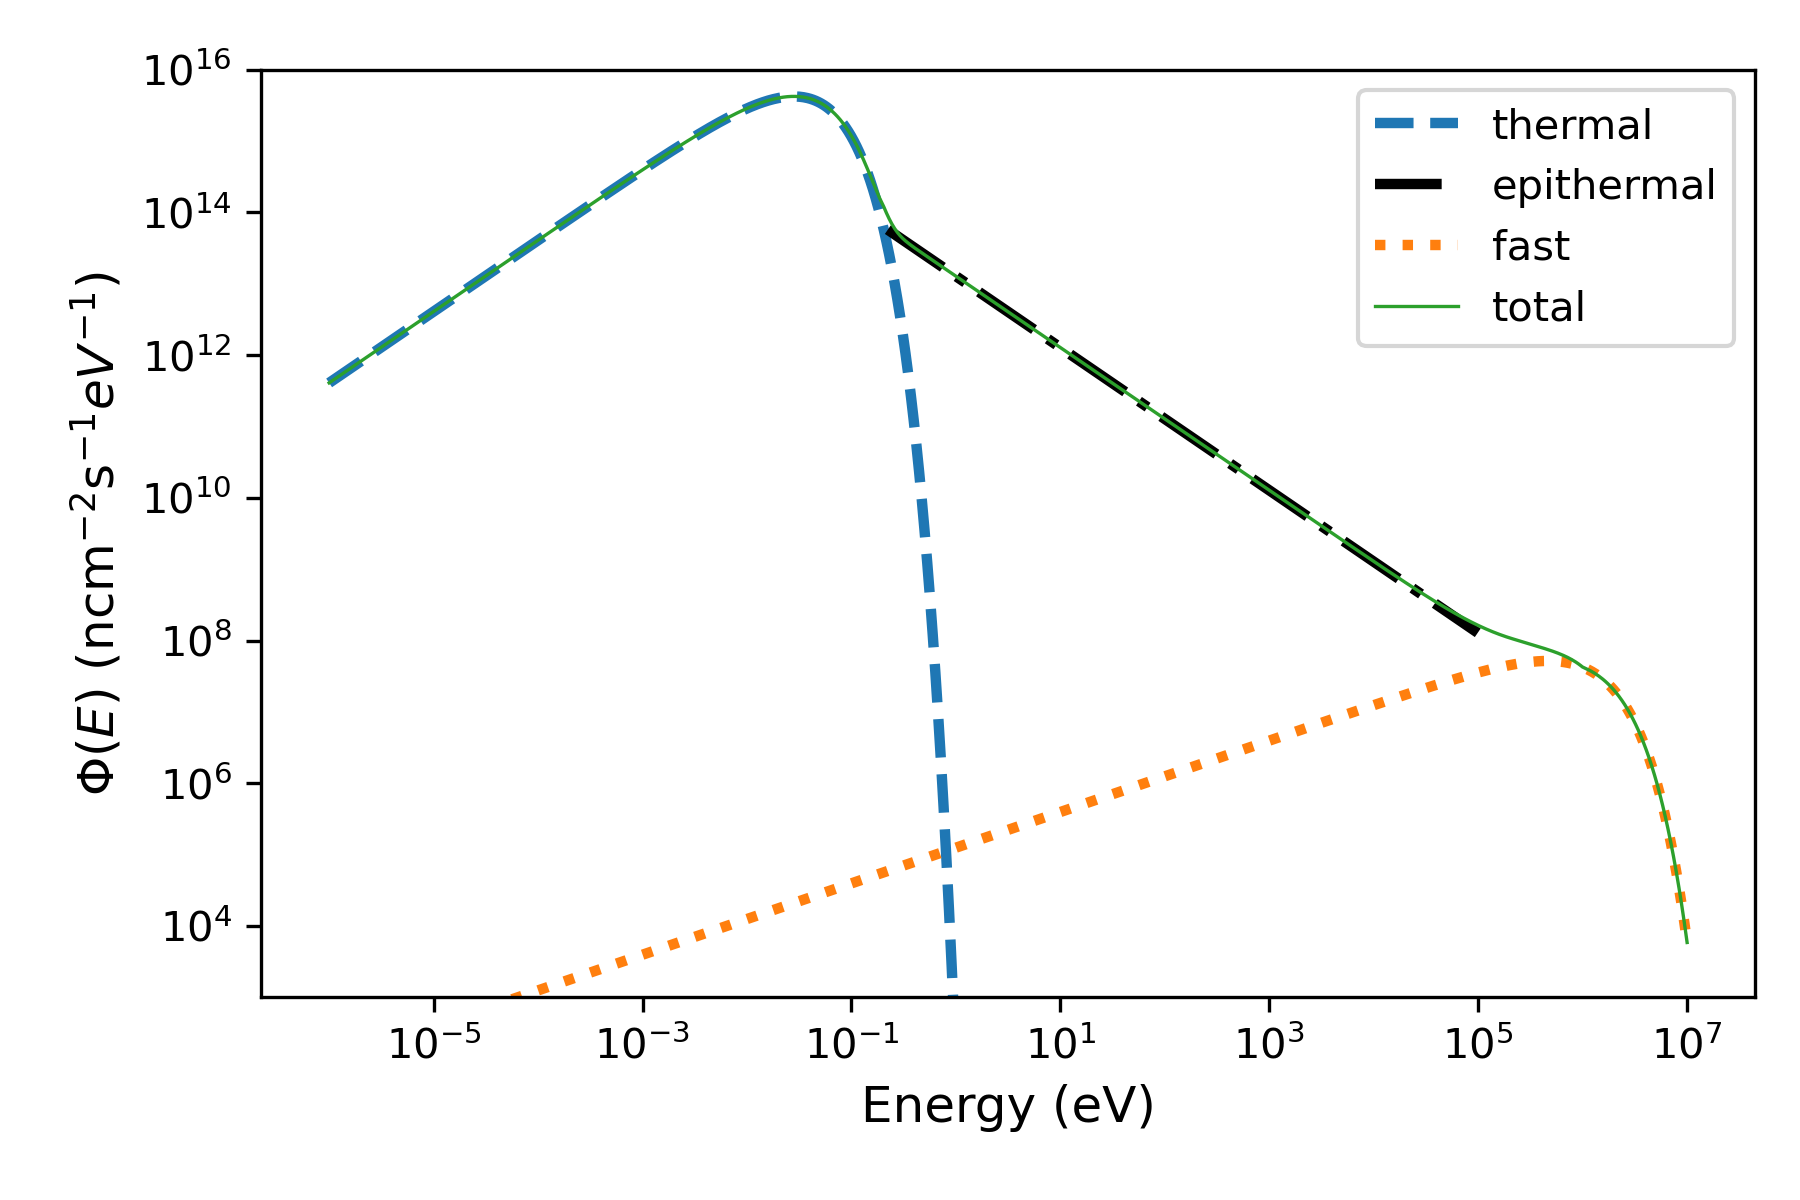
\includegraphics[scale=0.44] {figures/03-theoryspectrum.png}
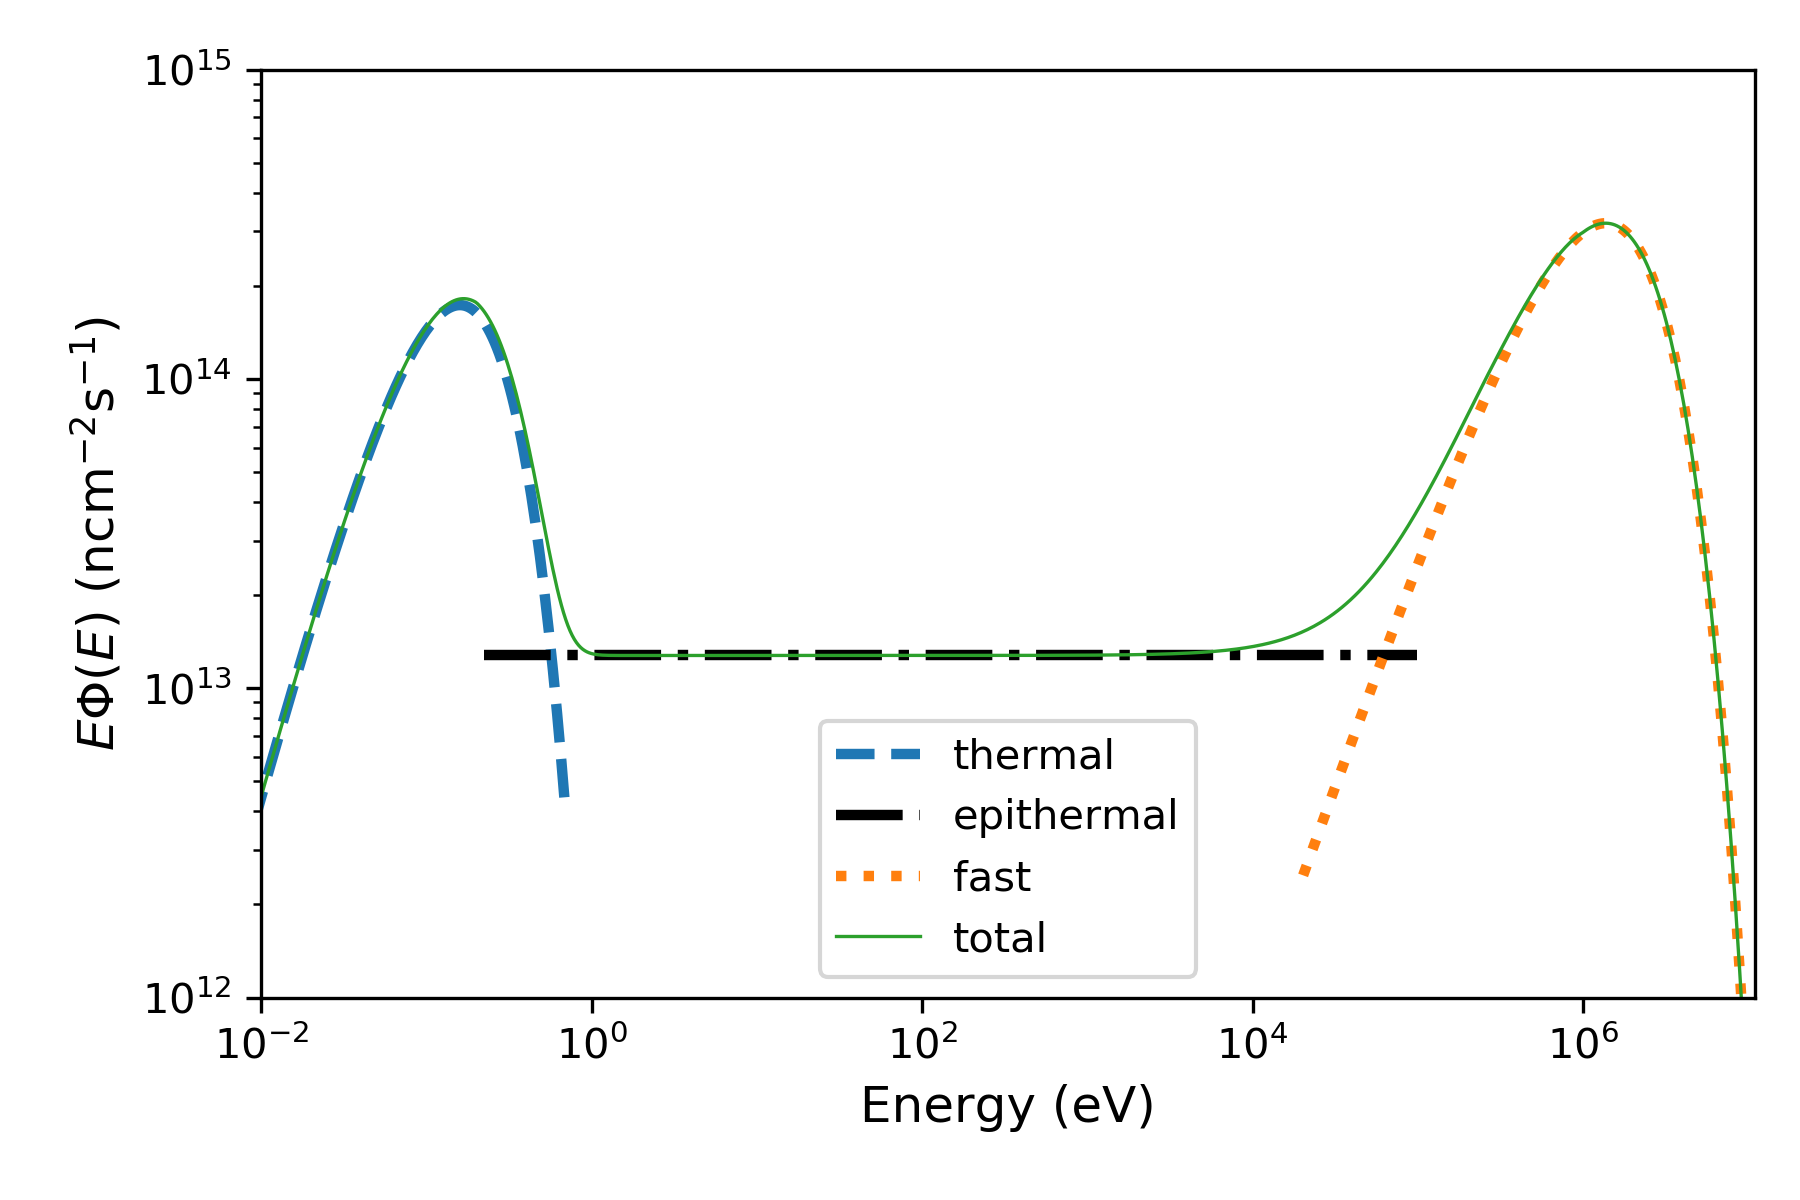
\includegraphics[scale=0.44] {figures/03-theoryspectrumlet.png}}\protect
\caption{\label{fig:idealneutronspectrum} \footnotesize{Idealized neutron spectrum.}}
\end{figure}

In the discussions of slowing down an other quantity is often introduces, the \textit{slowing down density}, which in our case is

$$q(E)=q(u)=\xi\Sigma_t\Phi(u)$$,

which gives the number of neutrons per unit time passing a certain lethargy (or energy). It is possible to give a more formal mathematical expression defining this quantity, and the interested reader is referred to D\&H (p321). However, we will your in our rather simplistic discussions.


\vspace{0.5cm}

\textbf{Slowing down on Hydrogen in the presence of absorbers}

Let us consider a case more relevant for reactor physics: a homogeneous mixture of hydrogen and heavy absorber nuclei (eg. uranium nuclei). We can notice from Table \ref{tab:moderator} that slowing down on the heavy nuclei can be neglected compared to the slowing down on hydrogen, thus in Eq. \eqref{eq:scatkernel} it is enough to consider hydrogen (for which $\alpha=0$) However, resonance absorption might occur when a neutron interacts with a heavy nucleus. 

With some laborious derivation (see for example Stacey's book) one can arrive to

\begin{equation}\label{eq:slowingdownHU}
 \Phi(E) = \frac{\Sigma_A^U(E_1) + \Sigma_S^H(E_1)}{ \Sigma_A^U(E) + \Sigma_S^H(E)} \cdot \frac{E_1\phi(E_1)}{E} \cdot \mathrm{exp}\left[-\int_E^{E_1} \frac{1}{E'} \frac{\Sigma_A^U(E')}{\Sigma_A^U(E') + \Sigma_S^H(E')}dE'\right]
\end{equation}

\noindent which gives a relation of the flux at $E$, to the flux at a higher energy $E_1$. First of all we can note that the lethargic flux at any energy is proportional to the lethargic flux at an other energy $\Phi(E)E \propto \phi(E_1)E_1$. And the proportionality is given by two factors: the first one is the ratio of the cross sections (absorption of uranium and scattering of hydrogen) at the respective energies; the second, exponential term which includes an integral from $E$ to $E_1$. The integral will always be positive therefore the exponential will be between 0 and 1, hence can be interpreted as a probability. 

We can consider three cases for $E$ and $E_1$:

1. The two energies are between resonances ($E_{r1}<E<E_1<E_{r2}$). Then the cross sections are close to constant, hence the first term $\approx 1$. And due to the scattering cross section of hydrogen is much larger than the absorption cross section of uranium, the exponent also becomes $\approx 1$. Therefore, we can conclude that  

$$\phi(E) \approx \frac{E_1\phi(E_1)}{E}$$

\noindent thus the lethargic flux is constant, and this is exactly what we have observed previously for the case when only scattering was considered.

2. When the energy is at a resonance $E_r=E<E_1$, the absorption cross section is much higher than the scattering. therefore the first term will become much smaller than 1. Since we know that the exponent is between 0 and 1, it will not influence our qualitative finding that 

$$\phi(E)E \ll \phi(E_1)E_1$$

\noindent the flux is greatly decreased at the resonance energy as illustrated in Figure~\ref{fig:selfshielding} for the notable resonance of U-238 at 6.67 eV. Neutrons that are scattered into the energy range of the resonance are absorbed, but those neutrons that scatter from energies above the resonances to energies below the resonances are not affected. However, due to the reduction in the flux, rate of resonance absorption also decreases, this is called \textit{energy self-shielding}.

\begin{figure}[ht!]
\protect \centering{
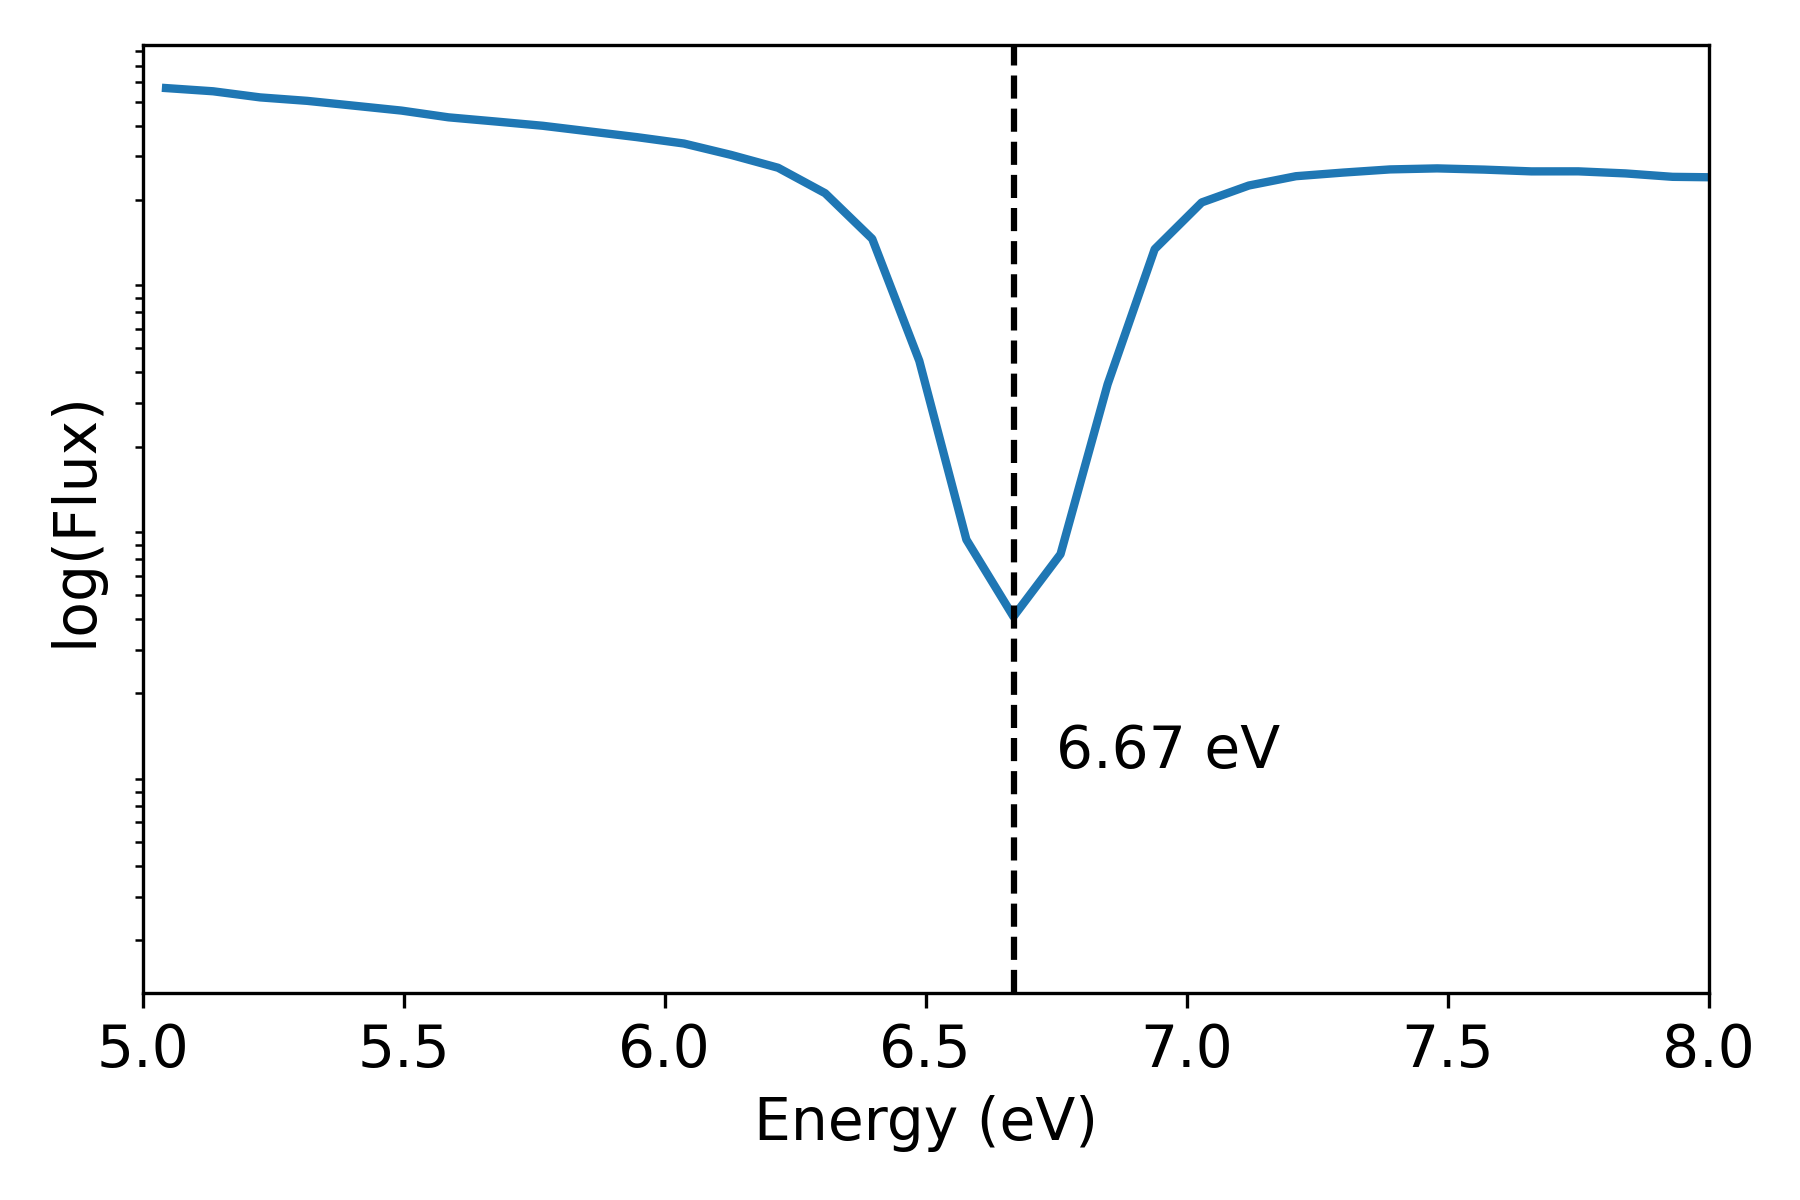
\includegraphics[scale=0.44] {figures/02-selfshielding.png}}\protect
\caption{\label{fig:selfshielding} \footnotesize{Resonance self-shielding.}}
\end{figure}
 
\begin{figure}[ht!]
\protect \centering{
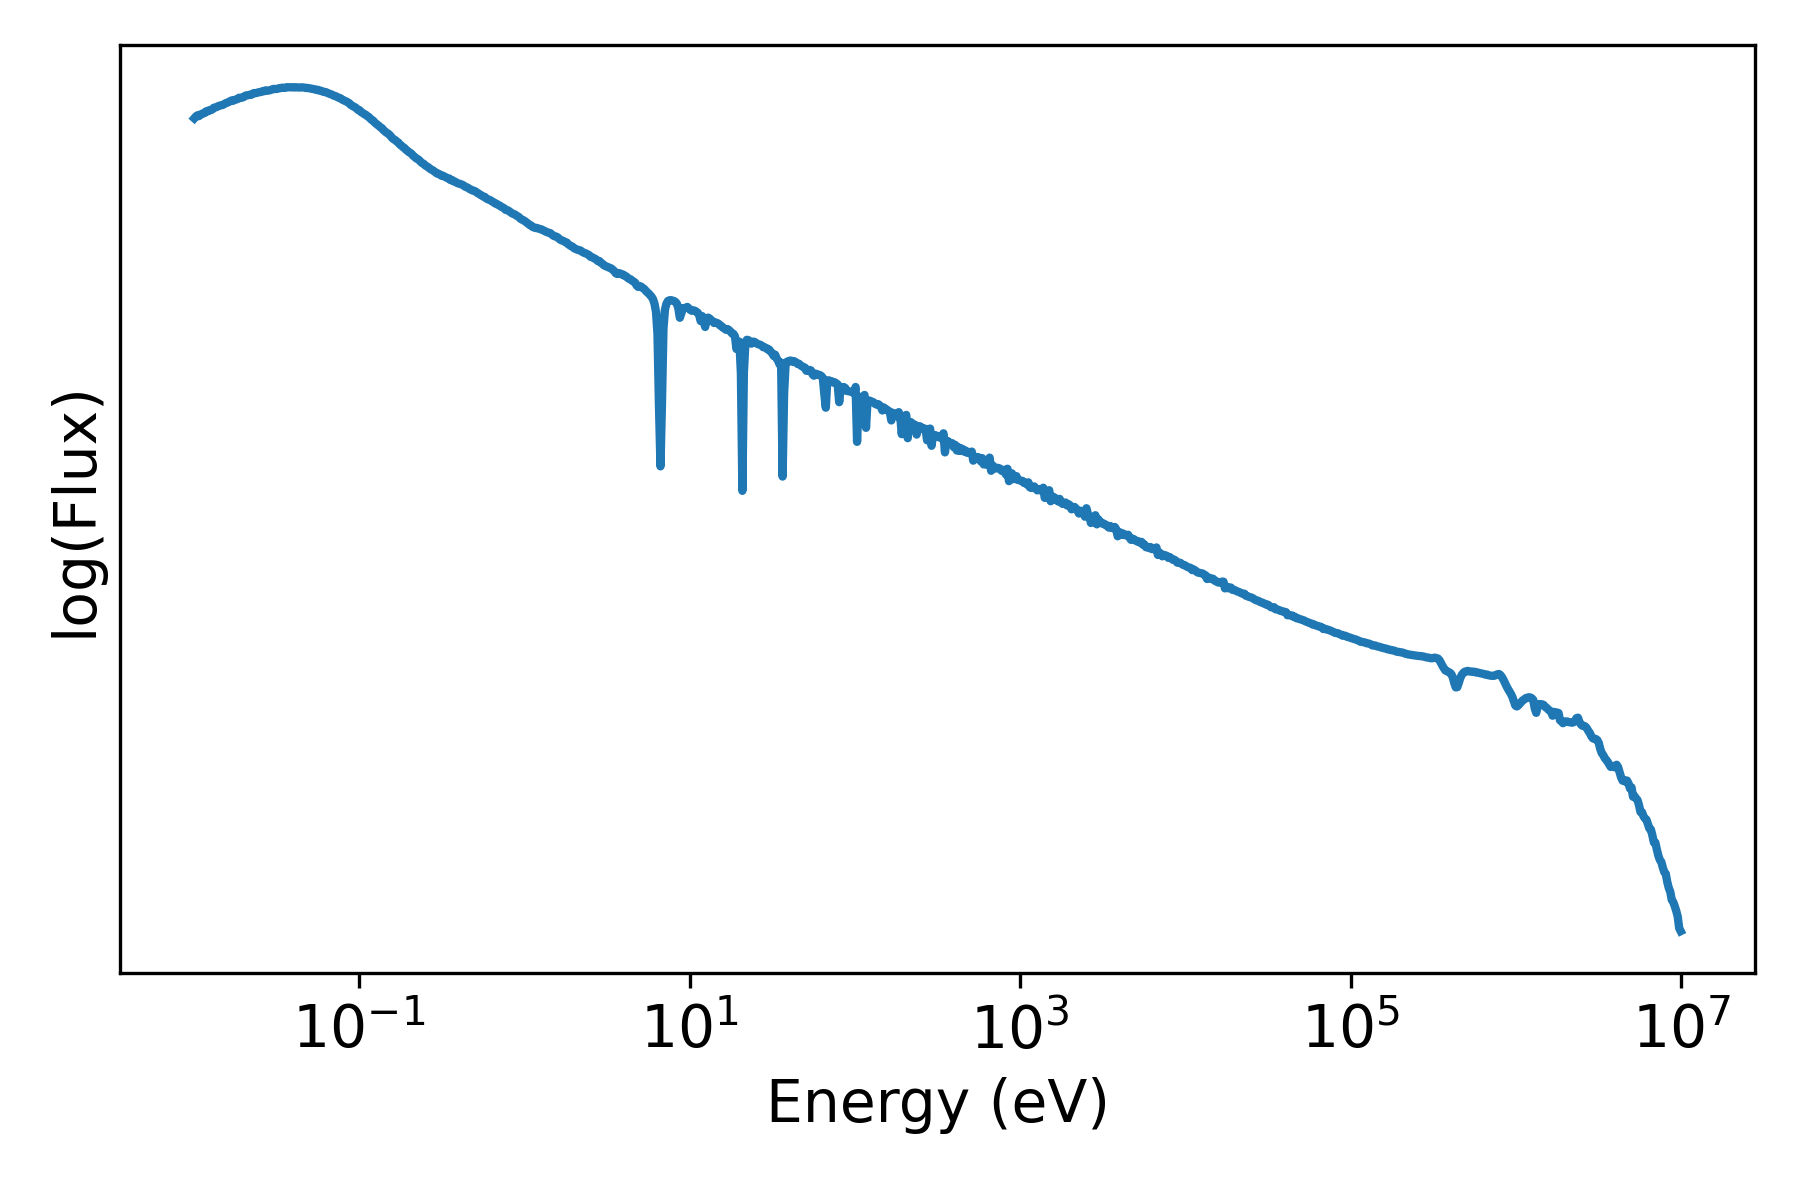
\includegraphics[scale=0.44] {figures/02-pwrspectrum.png}
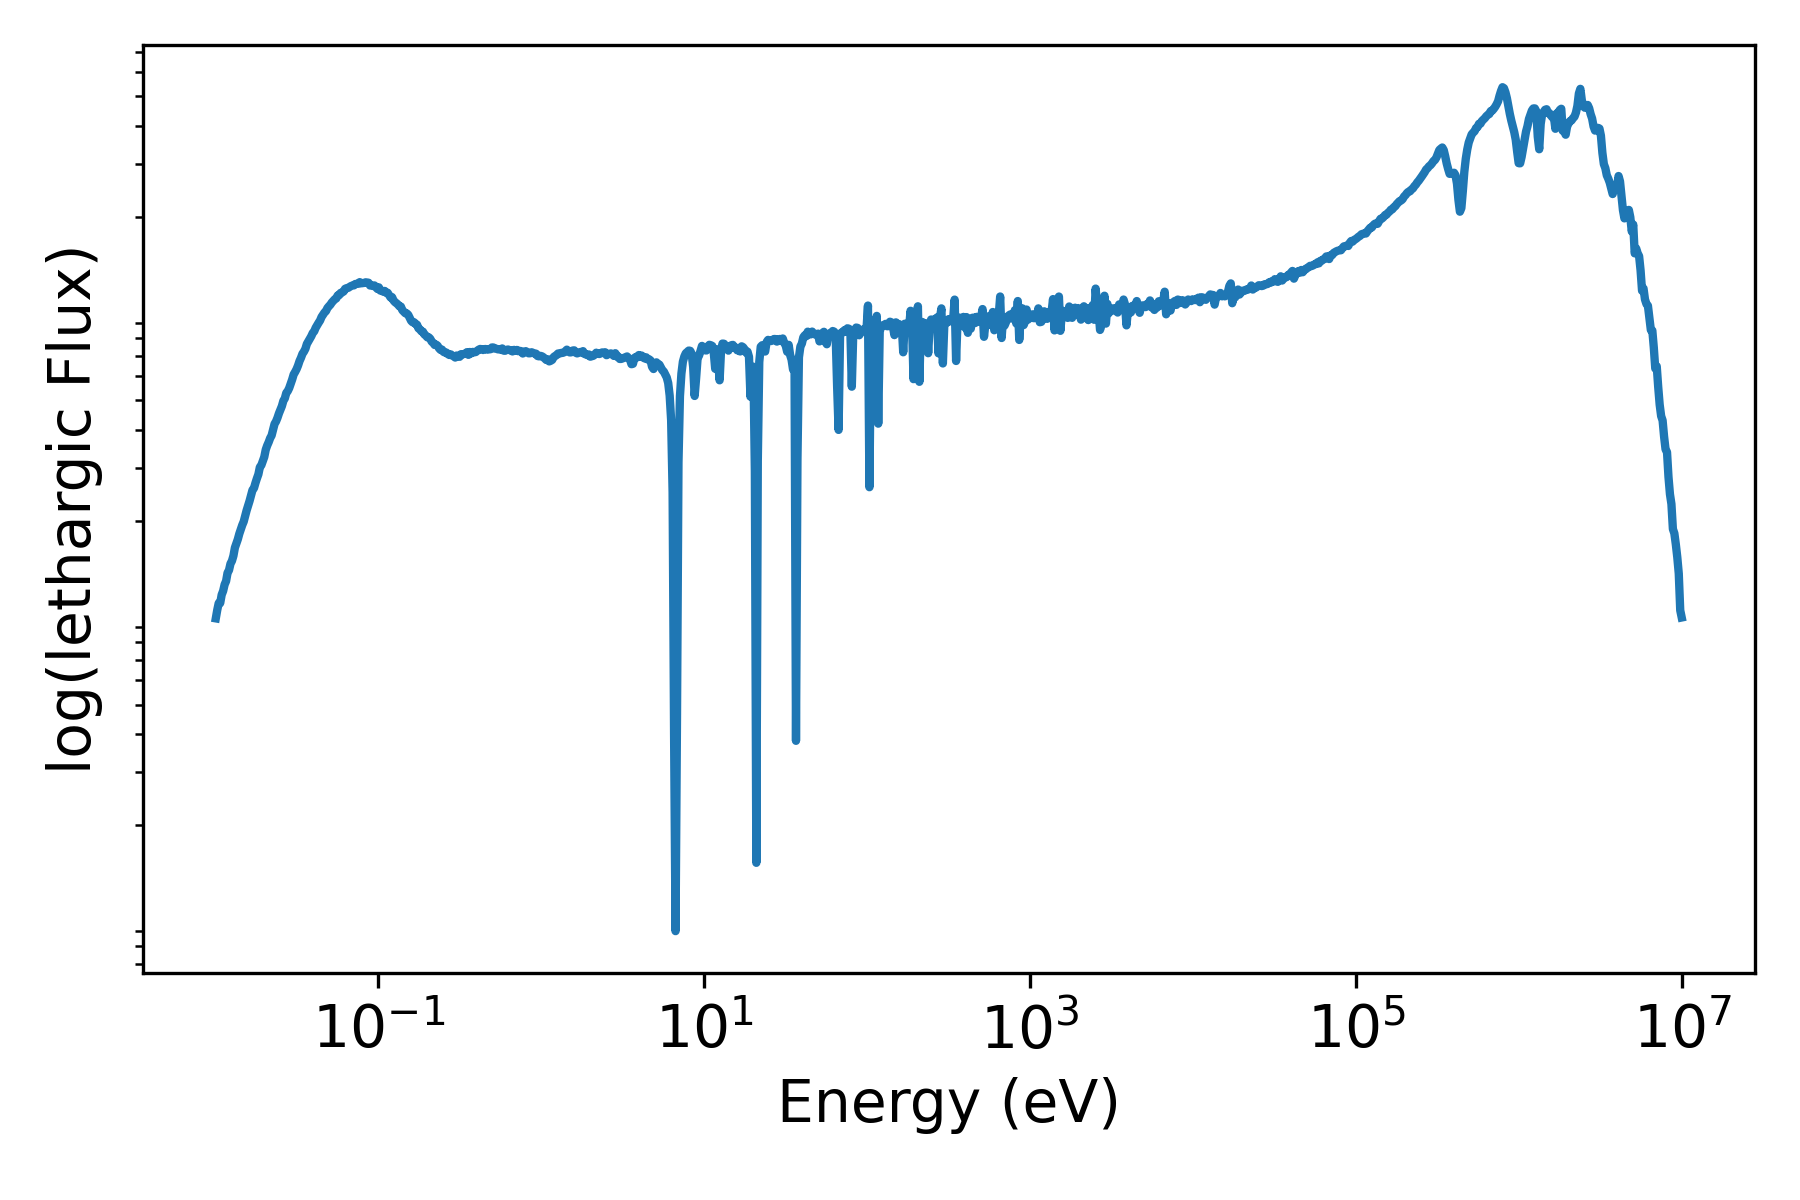
\includegraphics[scale=0.44] {figures/02-pwrspectrumlethargic.png}}\protect
\caption{\label{fig:realneutronspectrum} \footnotesize{PWR neutron spectrum ($\Phi(E)$ and $E\Phi(E)$).}}
\end{figure}

3. When the energies are separated by a resonance $E<E_r<E_1$, the first term is again close to unity, however the exponent is slightly less than~1 depending on the resonance width, which implies that the neutron flux is lower at the low energy side of the resonance compared to the high energy side. This is called \textit{resonance shielding}.

Figure \ref{fig:realneutronspectrum} illustrates the spectrum and the lethargic spectrum for a PWR calculation. We can recognize the above mentioned regions: Maxwell-distribution at thermal energies, the source Watt-distribution at fast energies with some influence from inelastic scattering, the close to $1/E$ trend in the slowing down region with the self-shielding effects.

\subsubsection{Resonance escape probability}

The probability appearing in Eq. \eqref{eq:slowingdownHU} if integrated over several resonances 

$$p(E_S\rightarrow E)=\exp\Bigg(-\int\limits_E^{E_S}\frac{\Sigma_a(E')}{E'\Sigma_t(E')}dE'\Bigg)$$

is called resonance escape probability, because it gives the ratio of neutrons which were not absorbed by the resonances while slowing down from $E_S$ to $E$.

$$\frac{S-\int\limits_E^{E_s}\Sigma_a(E')\Phi(E')dE'}{S}=p(E_S\rightarrow E)$$

Let's recall the phenomena of Doppler-broadening (ie. that the height of the resonance decreases while the width of the resonance increases with temperature), although the area under the resonance is constant, neutrons slowing down in discrete steps will have a higher probability to interact with the resonance, therefore the resonance escape probability $p$ decreases as the temperature increases. This, as we will see later when discussing feedback mechanisms, has an important implication on reactor safety: with increasing power, therefore increasing temperature the negative feedback of the Doppler-effect reduces the power.

% FOR FUTURE: RESONANCE INTEGRALS!!!
%The slowing down equation \ref{eq:slowingdown} becomes
%
%$$\int\limits_E^{\infty} \Phi(E')\frac{\Sigma_s(E')}{E'}dE'+S(E)=\Sigma_t(E)\Phi(E)$$
%
%\noindent where $\Sigma_s$ includes only the moderator, but $\Sigma_a$ (hidden in $\Sigma_t$) includes both the moderator and the heavy absorber. After differentiation one arrives to
%
%$$\frac{dF(E)}{dE}+\frac{\Sigma_s(E)}{E\Sigma_t(E)}F(E)=\frac{dS(E)}{dE}$$
%
%\noindent with introducing again the collision density $F(E)=\Sigma_t(E)\Phi(E)$. Of course we need some initial conditions for the differential equation. This we can get by considering that the source might have a maximum energy $E_max$ (for a monoenergetic source this would be obvious, for the Watt-spectrum we can safely assume this to be 10 MeV). Therefore the absorption rate above this energy is
%
%$$\int_{E_{max}}^\infty\Sigma_a(E)\Phi(E)dE=0$$
%
%\noindent which requires the flux, and therefore the collision density to be zero above this energy.
%
%$$F(E)=0 \: \text{for} \: E\geq E_{max} $$
%
%Here we will omit deriving the solution (it can be found in books). Just present the rather involved result
%
%$$F(E)=S(E)+\frac{1}{E}\int\limits_E^\infty S(E')\frac{\Sigma_s(E')}{\Sigma_t(E')}\exp\Big(-\int\limits_E^{E'}\frac{\Sigma_a(E'')}{E''\Sigma_t(E'')}dE''\Big)dE'$$ 
%
%\noindent but as probably at this point we are already used to this, we can make some reasonable assumptions to simplify this result.

%As mentioned before, in our discussion we are going to make serious assumptions: we will be studying slowing down in an infinite medium where a monoenergetic source emits neutrons uniformly. We also consider that elastic scattering is isotropic (therefore, we know that our derivations will be close to reality only below 100 keV).
%
%When discussing slowing down it is convenient to introduce two quantities:
%
%$$F(E)=\Sigma_S(E)\phi(E)=\text{collision density}$$
%
%\noindent which gives the number of collision per unit volume, unit time and unit energy in the energy bin $[E,E+dE]$. Notice that in fact this is a reaction rate-like quantity.
%
%$$q(E)=\text{slowing-down density}$$
%
%\noindent which gives the number of neutrons per unit volume and per unit time whose energy falls below $E$.
%
%Then we will discuss slowing-down for two cases: without and with absorption. And we will assume that the energies are well below the energy of the source.  We also require for the derivation that we are in the asymptotic region ($E<\alpha^3E_0)$), since close to the energy of the source, it is undetermined how many collisions are required to reach energy $E$. It might take one or more collisions. However, energies well below the source energy, we can assume that neutrons cannot reach directly.


\subsection{Neutron cycle: 4 factor formula}

We have previously developed a simple $2 factor$ model to estimate the multiplication factor $k$. Since then however we have studied the neutron spectrum, and discussed how neutrons are slowing down, and if they escape the resonance region then might reach thermal energies and cause fission, therefore we can give a more appropriate model for the neutron cycle that is when neutrons are born in fission, slow down, and might initiate fission thus giving birth to a new generation of neutrons as being illustrated in Figure \ref{fig:neutroncycle}.

Up to now we have considered homogeneous reactors, but in order to accommodate that in actual reactors the fuel and the moderating material is well separated (for an LWR in the form of fuel rods and coolant channels), we will consider a space and energy dependent flux $\phi(\mathbf{r},E)$ in the following.

\begin{figure}[ht!]
\protect \centering{
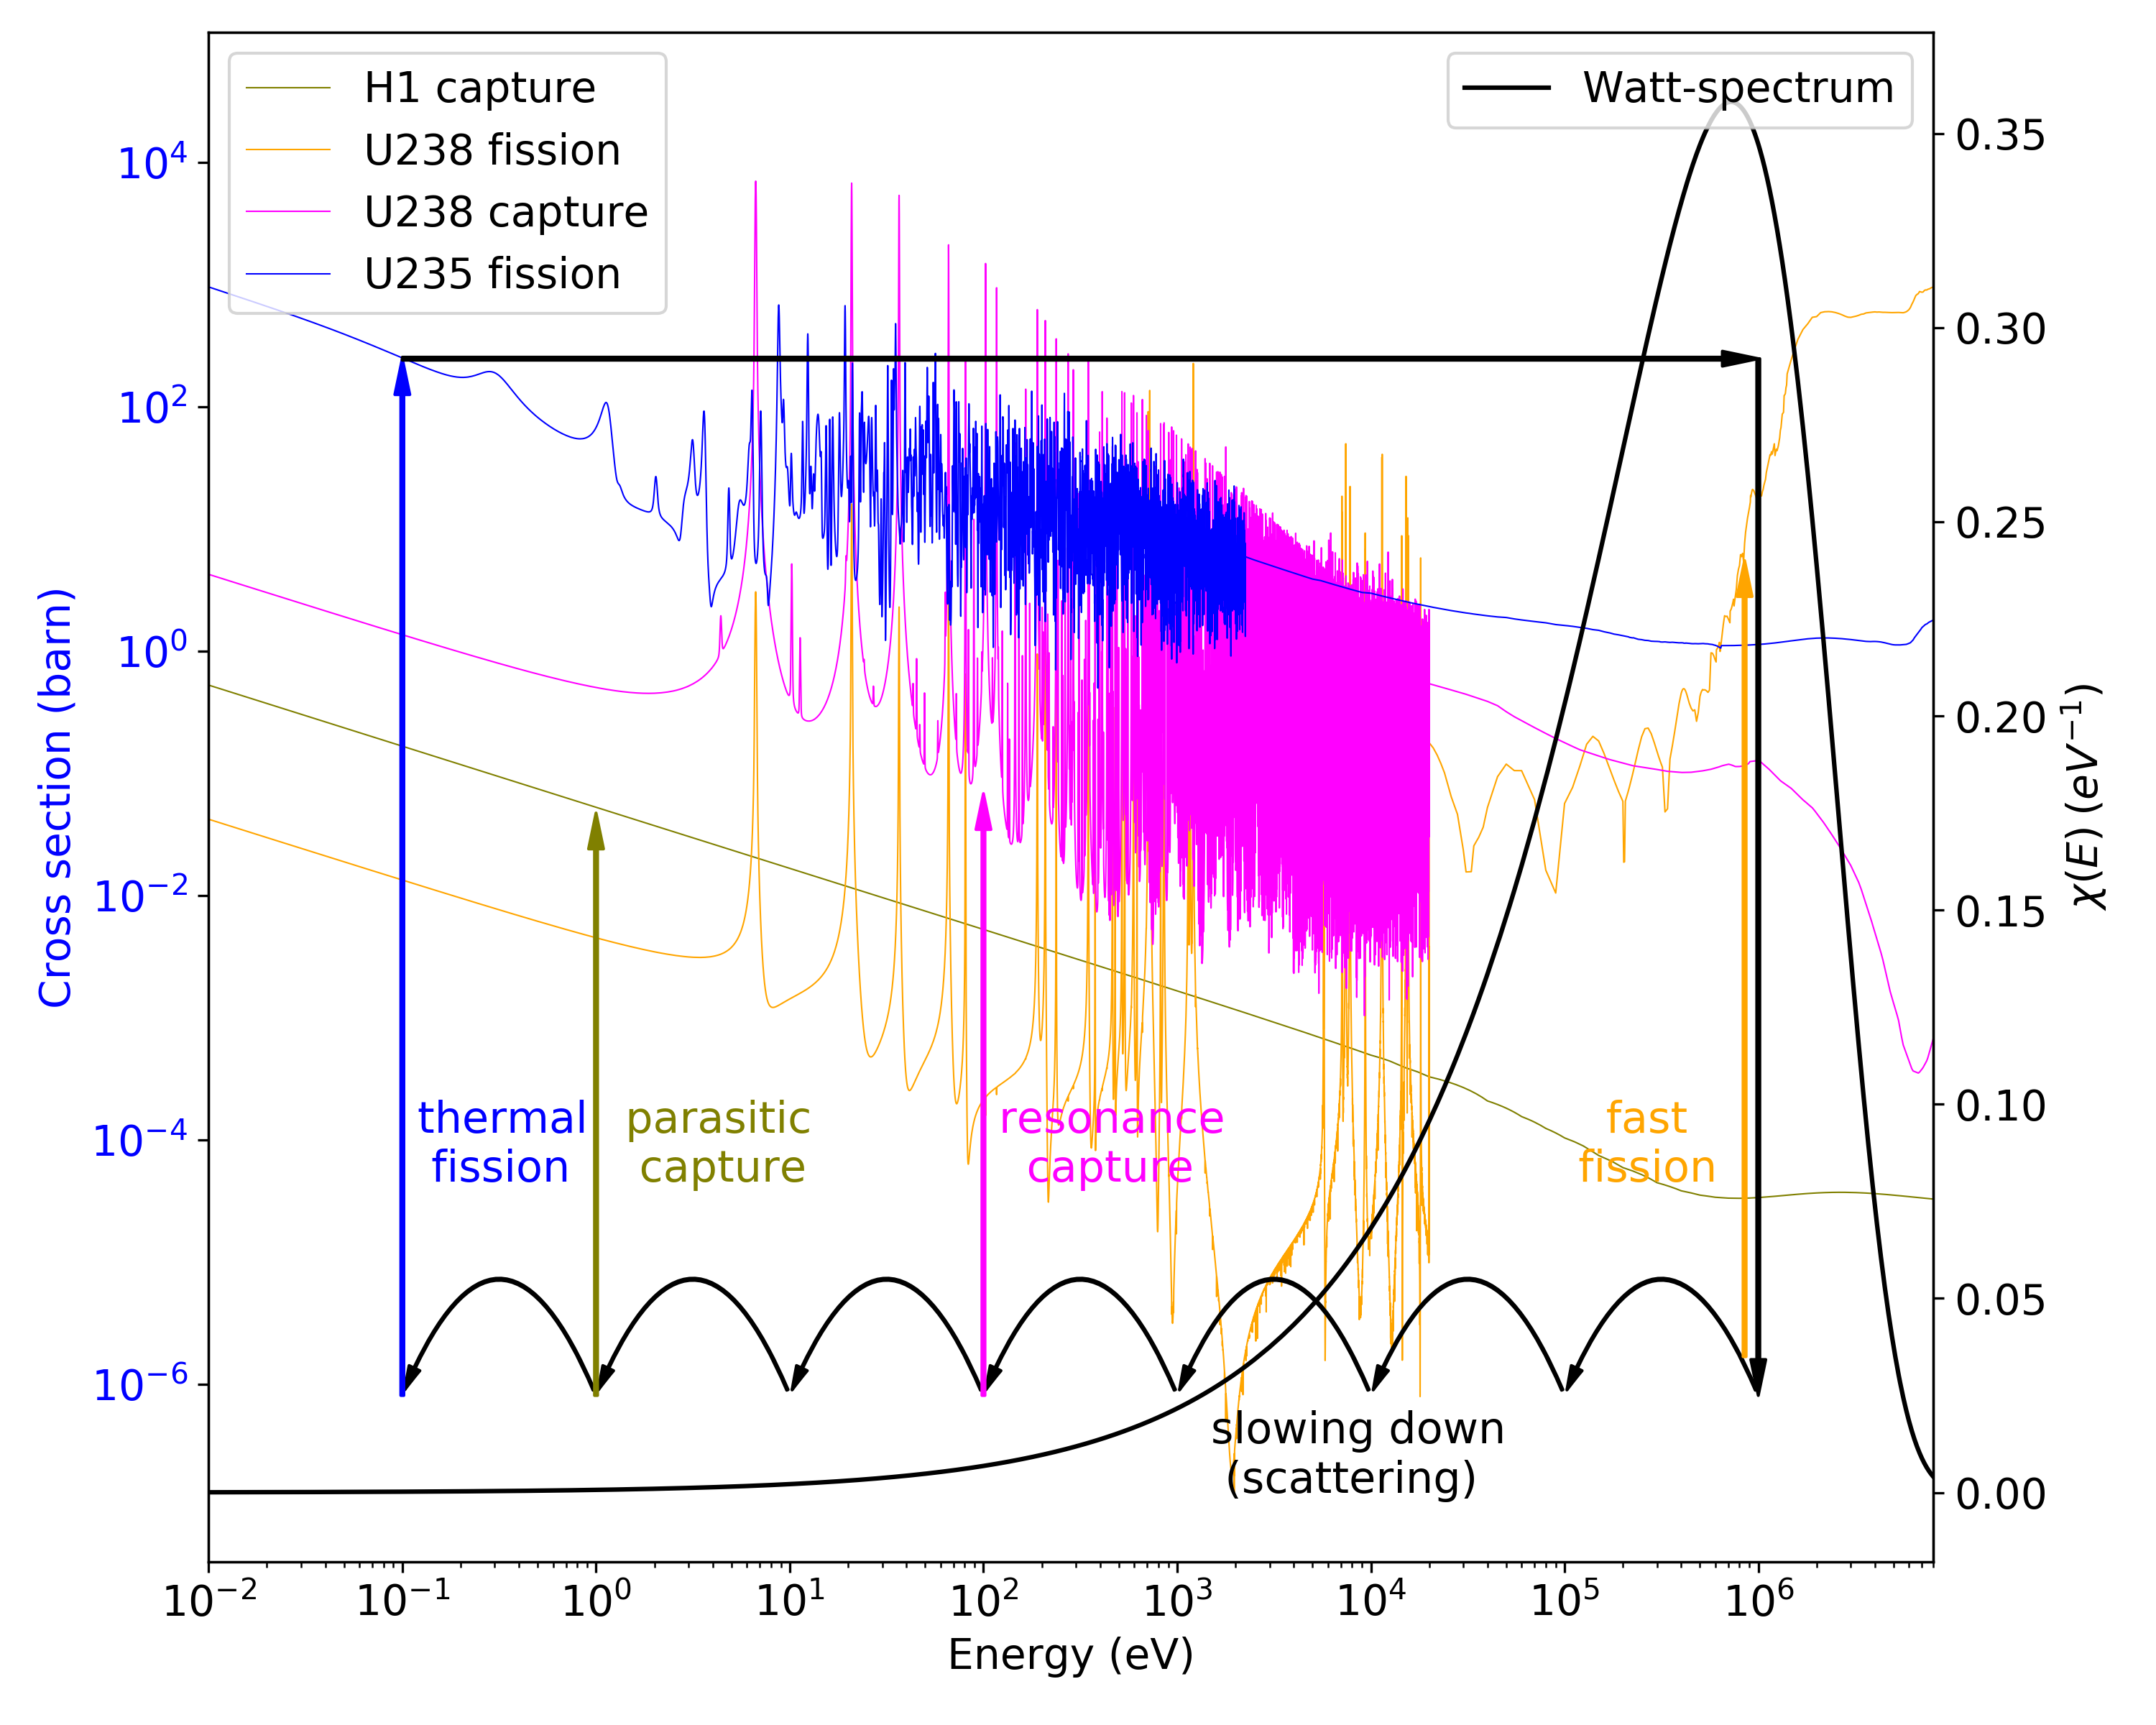
\includegraphics[scale=0.54] {figures/03-neutroncycle.png}}\protect
\caption{\label{fig:neutroncycle} \footnotesize{Schematic representation of the neutron cycle.}}
\end{figure}

At the beginning of the cycle neutrons are born at high energies. As we have previously noted, certain nuclides such as U-238 have a threshold for fission with high energy neutrons, thus in fact some of the neutrons are born due to fast fission. This is characterized by the \textit{fast fission factor}, 

$$\epsilon=\frac{\int_{V_{F}} \int_0^\infty \nu(E)\Sigma_f(\mathbf{r},E)\phi(\mathbf{r},E)dVdE}{\int_{V_{F}} \int_0^{\sim 5kT} \nu(E)\Sigma_f(\mathbf{r},E)\phi(\mathbf{r},E)dVdE}$$

\noindent which characterizes the ratio of the number of neutrons born in fission (due to both thermal and fast neutrons) and the number of neutrons born in fission induced by thermal neutrons.

Then, after birth the neutrons will slow down mainly due to elastic scattering events. The \textit{resonance escape probability} 

$$p=1-\frac{\int_{V_{F}} \int_{\sim 5kT}^\infty \Sigma_a(\mathbf{r},E)\phi(\mathbf{r},E)dVdE}{\int_{V_{F}} \int_0^{\infty} \nu(E)\Sigma_f(\mathbf{r},E)\phi(\mathbf{r},E)dVdE}$$

\noindent characterizes the probability that neutrons while traveling through the epithermal region will not be absorbed by the resonances of the absorber nuclei. 

When the neutrons reach the thermal region, due to the $1/v$-behavior of the cross sections they will be absorbed either in the fuel or due to parasitic capture of other materials (eg. coolant or structural elements. As we saw earlier, the \textit{thermal utilization factor}

$$f=\frac{\int_{V_{F}} \int_0^{\sim 5kT} \Sigma_a(\mathbf{r},E)\phi(\mathbf{r},E)dVdE}{\int_{V_{total}} \int_0^{\sim 5kT} \Sigma_a(\mathbf{r},E)\phi(\mathbf{r},E)dVdE}$$

characterizes the ratio of the number of thermal neutrons absorbed in the fuel and the number of thermal neutrons absorbed in other materials.

Finally, neutrons which are absorbed by the fuel might induce fission from which new neutrons emerge or are captured by the nuclei. The \textit{thermal fission factor}

$$\eta=\frac{\int_{V_{F}} \int_0^{\sim 5kT} \nu(E)\Sigma_f(\mathbf{r},E)\phi(\mathbf{r},E)dVdE}{\int_{V_{F}} \int_0^{\sim 5kT} \Sigma_a(\mathbf{r},E)\phi(\mathbf{r},E)dVdE}$$

gives the average number of fission neutrons emitted per thermal neutron absorbed in the fuel.

By multiplying these values we can calculate the infinite multiplication factor through the \textit{4-factor formula}

$$k_{\infty}=\eta f p \epsilon$$

In order to compute the k-effective, one needs to take into account the leakage, which is often given denoted separately for fast and thermal neutrons: $P_{FNL}$, $P_{TNL}$. However, it has to be highlighted again, that the determination of the non-leakage probabilities is rather complicated.

Today, the 4-factor formula is rather an educational tool to summarize the various processes in fission chain reactions, or to illustrate the impact of changing some parameter of the reactor (eq. temperature), and in practice it has little use. Nevertheless, before computers could have been used for elaborate calculations, this formula was the basis of reactor physics: the factors were determined from measurements, and then the formula was used to determine the multiplication factor.

However, as we will see in the next Chapter, today we can use more elaborate methods to estimate the multiplication factor.

%\end{document}